\documentclass[conference,letterpaper]{IEEEtran}
\IEEEoverridecommandlockouts

% ===================== PACKAGES =====================
\usepackage{cite}
\usepackage{amsmath,amssymb,amsfonts}
\usepackage{algorithmic}
\usepackage{graphicx}
\usepackage{textcomp}
\usepackage{xcolor}
\usepackage{url}
\usepackage{float}
\usepackage{algorithm}
\usepackage{array}
\usepackage{booktabs}
\usepackage{multirow}
\usepackage{enumitem}
\ifCLASSOPTIONcompsoc
  \usepackage[caption=false,font=normalsize,labelfont=sf,textfont=sf]{subfig}
\else
  \usepackage[caption=false,font=footnotesize]{subfig}
\fi

% Spacing parameters for clean, uncluttered IEEE layout
\setlength{\columnsep}{0.25in}
\setlength{\intextsep}{10pt plus 2pt minus 2pt}
\setlength{\textfloatsep}{12pt plus 2pt minus 2pt}
\setlength{\floatsep}{10pt plus 2pt minus 2pt}
\renewcommand{\arraystretch}{1.20}
\renewcommand{\algorithmicrequire}{\textbf{Input:}}
\renewcommand{\algorithmicensure}{\textbf{Output:}}

% Tighten itemize and enumerate indentation to eliminate sidebar gaps in 2-column format
\setlist[itemize]{leftmargin=1.2em, itemsep=2pt, topsep=2pt, parsep=0pt}
\setlist[enumerate]{leftmargin=1.4em, itemsep=2pt, topsep=2pt, parsep=0pt, label=\arabic*)}

\def\BibTeX{{\rm B\kern-.05em{\sc i\kern-.025em b}\kern-.08em
T\kern-.1667em\lower.7ex\hbox{E}\kern-.125emX}}

% ===================== AUTHOR LINE BREAK FIX =====================
\makeatletter
\newcommand{\linebreakand}{%
\end{@IEEEauthorhalign}
\hfill\mbox{}\par
\mbox{}\hfill\begin{@IEEEauthorhalign}
}
\makeatother

\flushbottom

\begin{document}

% ===================== TITLE =====================
\title{Adaptive Label-Efficient Cross-Sensor Hyperspectral Image Classification Framework Using Frozen Spectral Foundation Models}

% ===================== AUTHORS =====================
\author{
\IEEEauthorblockN{Dr. Arun Anoop M}
\IEEEauthorblockA{\textit{Department of Computer Science and Engineering} \\
\textit{AJ Institute of Engineering and Technology} \\
Karnataka, India \\
dr.arunanoop@ajiet.edu.in}
\and
\IEEEauthorblockN{Harinand Sreeshan}
\IEEEauthorblockA{\textit{Department of Computer Science and Engineering} \\
\textit{AJ Institute of Engineering and Technology} \\
Karnataka, India \\
harinandsreeshan@gmail.com}
\linebreakand
\IEEEauthorblockN{Ashik Krishnan}
\IEEEauthorblockA{\textit{Department of Computer Science and Engineering} \\
\textit{AJ Institute of Engineering and Technology} \\
Karnataka, India \\
ashikkrishnan72@gmail.com}
\and
\IEEEauthorblockN{Mrinal Ramachandran}
\IEEEauthorblockA{\textit{Department of Computer Science and Engineering} \\
\textit{AJ Institute of Engineering and Technology} \\
Karnataka, India \\
mrinalramachandran012@gmail.com}
\linebreakand
\IEEEauthorblockN{Arjun Sasi}
\IEEEauthorblockA{\textit{Department of Computer Science and Engineering} \\
\textit{AJ Institute of Engineering and Technology} \\
Karnataka, India \\
arjunsasi1423@gmail.com}
}

\maketitle

% ===================== ABSTRACT =====================
\begin{abstract}
Hyperspectral image (HSI) classification is a cornerstone of quantitative remote sensing, facilitating fine-grained material identification for precision agriculture, environmental surveillance, mineral exploration, and urban planning. While recent transformer models and large-scale hyperspectral foundation models achieve high classification accuracy, they routinely demand abundant annotated pixels and impose substantial computational overhead during end-to-end retraining, frequently succumbing to catastrophic forgetting and small-sample overfitting under tight labeling budgets. Furthermore, cross-sensor domain shifts with mismatched spectral channels severely inhibit the practical reusability of trained networks. 

\vspace{0.3em}
This paper presents an Adaptive Label-Efficient Cross-Sensor Hyperspectral Image Classification Framework built upon a frozen spectral foundation model paradigm. The proposed framework evaluates candidate hyperspectral backbones and establishes SpectralEarth (a 3D-ResNet architecture pretrained on 1.2 million unlabeled patches) as a permanently frozen feature extractor ($24.24\times 10^6$ parameters, 0 gradients), extracting expressive 2048-dimensional embeddings. A lightweight multilayer perceptron classifier head ($5.33\times 10^5$ parameters, representing only 2.15\% of total system parameters) is trained exclusively on the extracted representations. To accelerate active query rounds, an in-memory feature cache stores candidate representations once, reducing per-round feature extraction latency from 7.733\,s to 0.0919\,s (an $84.13\times$ speedup, and up to $2845.2\times$ per patch) with exact mathematical identity. 

\vspace{0.3em}
To minimize manual annotation effort without compromising accuracy, an intelligent active learning engine integrates post-hoc validation temperature scaling with candidate-filtered farthest-first diversity traversal. Rigorous 5-seed benchmark evaluations across Indian Pines, Salinas, and Pavia University demonstrate that the proposed framework delivers up to 23.1\% label savings (sparing 60 human annotations to achieve 60\% Overall Accuracy on Indian Pines) and decreases Expected Calibration Error by 43.8\% to 50.3\%. A controlled 90-run ablation study reveals that blindly stacking regularizers such as dropout and class weights induces negative gradient interactions ($p = 0.0288$ degradation on Salinas), demonstrating the empirical superiority of a clean, calibrated query design. For cross-sensor adaptation, deterministic 1D spectral resampling paired with classifier weight reuse enables AVIRIS-to-ROSIS transfer, achieving 49.84\%--54.12\% zero-shot Overall Accuracy and reaching 61.80\% with only 190 target-annotated samples. An interactive web-based demonstration system verifies the entire human-in-the-loop lifecycle under strict zero-leakage conditions.
\end{abstract}

\begin{IEEEkeywords}
Hyperspectral Image Classification, Spectral Foundation Models, Active Learning, Model Calibration, Temperature Scaling, Feature Caching, Cross-Sensor Adaptation, Remote Sensing.
\end{IEEEkeywords}

% ===================== INTRODUCTION =====================
\section{Introduction}

Hyperspectral imaging (HSI) acquires contiguous narrow spectral bands across electromagnetic wavelengths for every spatial pixel, capturing fine diagnostic absorption and reflectance signatures. This capability makes HSI indispensable for precision agriculture, forest canopy health monitoring, mineral mapping, disaster assessment, and defense applications \cite{roy2020,tuia2016}. However, processing hyperspectral data involves fundamental challenges: high spectral dimensionality, spatial-spectral autocorrelation, extreme ground-truth annotation scarcity, and severe distribution shifts across different remote sensing sensors.

\vspace{0.3em}
In recent years, deep learning has advanced HSI analysis through 3D/2D convolutional neural networks (e.g., HybridSN \cite{roy2020}) and vision transformers (e.g., SpectralFormer \cite{hong2022}, SSFTT \cite{he2022}). More recently, self-supervised hyperspectral foundation models, such as SpectralEarth \cite{braham2025} and HyperSIGMA \cite{wang2025}, have been pretrained on millions of unlabeled hyperspectral patches, demonstrating strong transferability. Despite their representational capacity, three primary bottlenecks prevent their practical deployment in operational remote sensing:

\begin{enumerate}
    \item \textbf{Prohibitive Annotation Cost and Small-Sample Overfitting:} Standard fine-tuning practices adapt all foundation model parameters on target scenes. When target annotations are scarce (e.g., fewer than 20 samples per class), updating tens of millions of parameters causes severe overfitting, loss of pretrained generalization, and training instability \cite{camps2021}.
    \item \textbf{Computational Burden in Iterative Workflows:} Active learning iteratively requests annotations for informative pixels. Retraining large foundation backbones at every active learning query round incurs prohibitive latency, preventing real-time human-in-the-loop interaction.
    \item \textbf{Miscalibration and Cross-Sensor Channel Mismatch:} Deep networks notoriously generate overconfident and miscalibrated posterior probabilities on small training pools, distorting uncertainty-based active query selection. Additionally, disparate sensor configurations (e.g., 200/204 bands for AVIRIS versus 103 bands for ROSIS) create channel incompatibilities that prevent direct model transfer.
\end{enumerate}

\vspace{0.3em}
To resolve these challenges simultaneously, this paper presents an \textit{Adaptive Label-Efficient Cross-Sensor Hyperspectral Image Classification Framework} using frozen spectral foundation representations, validation logit calibration, and candidate-filtered diversity selection. Rather than fine-tuning the complete backbone, we decouple feature extraction from task adaptation. The pretrained foundation backbone is kept 100\% frozen as an invariant feature extractor, generating 2048-dimensional embeddings that are cached in memory. A lightweight 2-layer multilayer perceptron (MLP) head is trained on these embeddings, updating merely 2.15\% of the total parameters in fractions of a second. Active querying is governed by validation-calibrated Least Confidence filtering coupled with farthest-first diversity traversal in feature space.

\begin{figure*}[t]
\centering
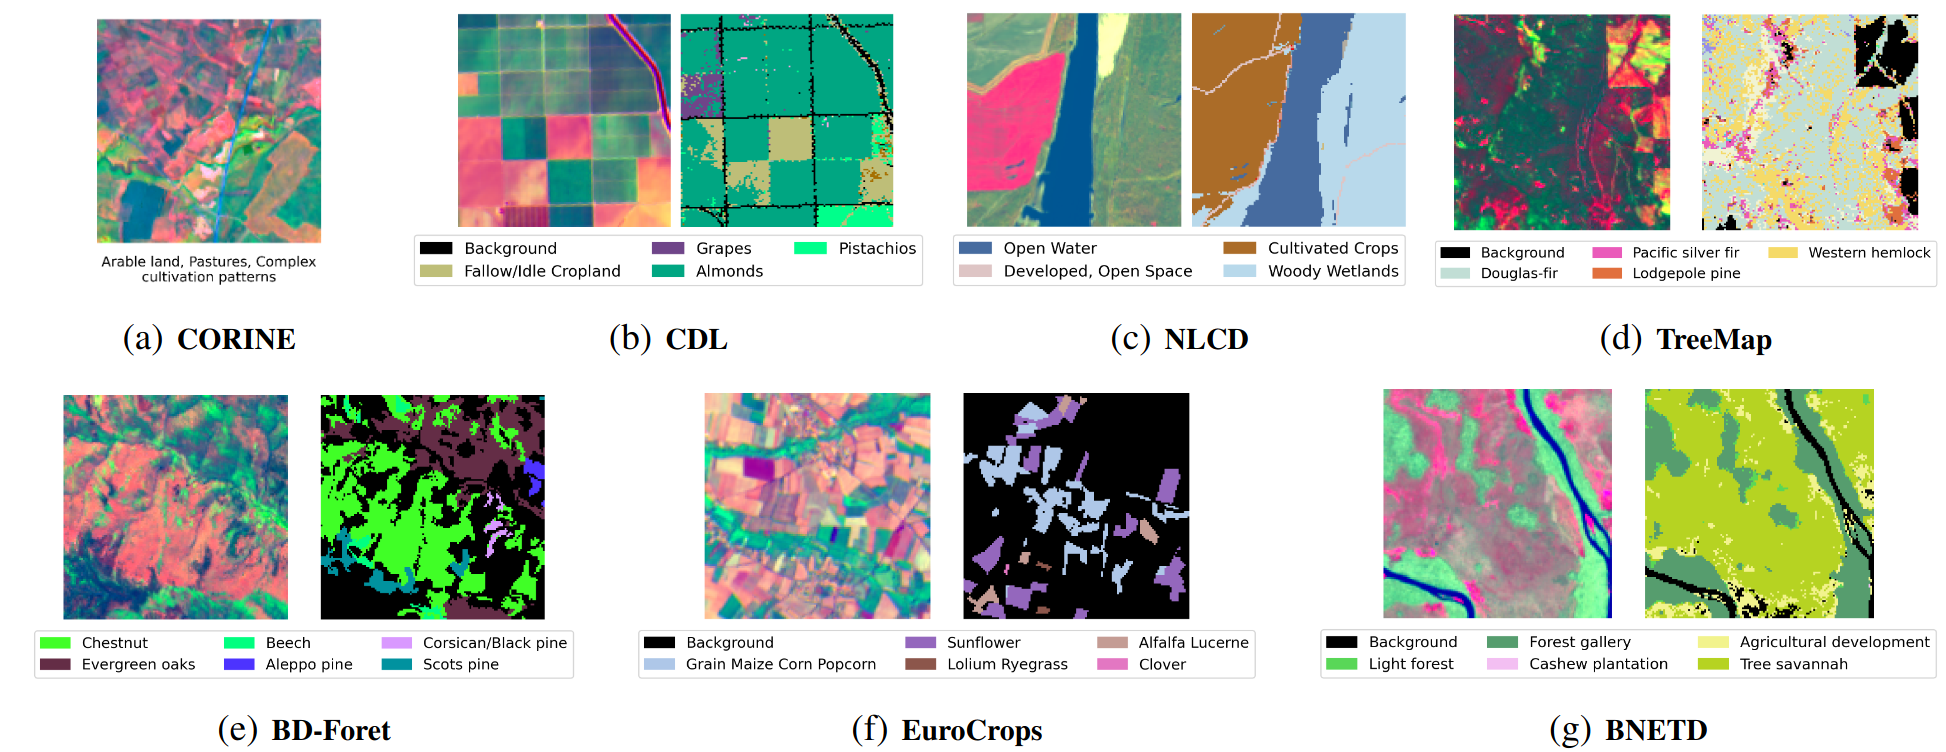
\includegraphics[width=\textwidth]{downstream_tasks_overview.png}
\caption{System architecture of the proposed Adaptive Label-Efficient Hyperspectral Framework, detailing frozen foundation backbone feature extraction, in-memory feature caching, lightweight classification, validation temperature calibration, active query selection, and cross-sensor deterministic adaptation.}
\label{fig:framework_architecture}
\end{figure*}

\subsection{Key Contributions}
The verified contributions of this work are summarized as follows:
\begin{itemize}
    \item \textbf{Frozen Foundation Model Paradigm with Zero-Overhead Caching:} We demonstrate that freezing a pretrained hyperspectral foundation backbone (`spec\_resnet50`, $24.24\times 10^6$ parameters) and training a lightweight 2-layer MLP head ($5.33\times 10^5$ parameters) achieves competitive classification accuracy while updating only 2.15\% of total system parameters. In-memory feature caching accelerates per-round feature extraction from 7.733\,s to 0.0919\,s ($84.13\times$ speedup) with exact numerical identity ($0.0$ difference).
    \item \textbf{Calibrated Uncertainty and Feature-Space Diversity:} We introduce a query engine combining post-hoc validation temperature scaling with candidate-filtered farthest-first traversal. On Indian Pines, this yields up to 23.1\% label savings (saving 60 human annotations to reach 60\% Overall Accuracy compared to random sampling) while cutting Expected Calibration Error (ECE) by 43.8\%--50.3\%.
    \item \textbf{Empirical Negative Interaction Proof via Ablation:} Across a controlled 5-seed, 90-run ablation suite, we empirically demonstrate that blindly stacking active learning enhancements (dropout, class-balanced loss, labeled-pool diversity) induces negative gradient interference and degrades Overall Accuracy ($p=0.0288$ on Salinas), justifying a clean, calibrated query design.
    \item \textbf{Deterministic Cross-Sensor Alignment and Adaptation:} We establish a zero-leakage cross-sensor adaptation protocol combining 1D linear spectral resampling (`SpectralResampler1D`) with classifier weight reuse, enabling AVIRIS-to-ROSIS transfer with 49.84\%--54.12\% zero-shot Overall Accuracy and rapid adaptation to 61.80\% within 190 target labels.
    \item \textbf{Interactive Human-in-the-Loop Demonstration:} We deploy an interactive web-based visualization system providing real-time sample inspections, uncertainty heatmaps, candidate rank explanations, and instantaneous retraining ($\approx 0.150$\,s).
\end{itemize}

% ===================== LITERATURE REVIEW =====================
\section{Related Work}

\subsection{Deep Hyperspectral Image Classification}
Early hyperspectral classification approaches relied on support vector machines (SVMs) and sparse representations \cite{tuia2011,li2013}. With deep learning, 2D and 3D convolutional architectures became dominant. HybridSN \cite{roy2020} combined 3D convolutions for joint spectral-spatial feature learning with 2D convolutions for spatial abstraction. Subsequently, vision transformers were adapted for hyperspectral data. SpectralFormer \cite{hong2022} and SSFTT \cite{he2022} modeled long-range spectral dependencies using self-attention. While effective, supervised deep models trained from scratch require substantial labeled data to prevent overfitting \cite{zhong2023}.

\subsection{Hyperspectral Foundation Models}
Foundation models pretrained on massive unlabeled earth observation datasets have emerged to address sample scarcity. SpectralEarth \cite{braham2025} trained a modified 3D-ResNet on 1.2 million hyperspectral patches using masked autoencoding, yielding generalizable spectral-spatial representations. Similarly, HyperSIGMA \cite{wang2025} explored foundation architectures across multiple remote sensing missions. However, the standard convention of fine-tuning foundation backbones remains computationally intensive and risks distorting pretrained representations when target labels are scarce.

\subsection{Active Learning in Remote Sensing}
Active learning (AL) seeks to minimize labeling costs by selectively querying the most informative unlabeled samples \cite{settles2009,tuia2016}. Classic uncertainty heuristics include entropy, margin sampling, and least confidence. To prevent querying redundant samples clustered around decision boundaries, diversity-aware methods incorporate feature-space clustering or core-set bounds \cite{sener2018}. BADGE \cite{ash2019} integrated uncertainty and diversity using gradient space embeddings with $k$-means++. However, backpropagating gradients through large backbones during AL rounds is computationally prohibitive. Table~\ref{tab:literature_comparison} situates our proposed framework relative to established literature.

\begin{table*}[!t]
\centering
\caption{Systematic Comparison of the Proposed Framework with Closest Related Literature}
\label{tab:literature_comparison}
\resizebox{\textwidth}{!}{%
\begin{tabular}{|l|c|c|c|c|c|c|}
\hline
\textbf{Property / Dimension} & \textbf{Tuia et al. \cite{tuia2011}} & \textbf{Li et al. \cite{li2013}} & \textbf{Sener \& Savarese \cite{sener2018}} & \textbf{Ash et al. \cite{ash2019}} & \textbf{Rasti et al. \cite{rasti2018}} & \textbf{Proposed SpectralEarth AL} \\
\hline
Backbone Architecture & Shallow SVM & Sparse Representation & ResNet18 (Scratch) & ResNet18 (Scratch) & Passive CNN & \textbf{Frozen SpecResNet50 ($24.24\times 10^6$)} \\
\hline
Trainable Parameters & N/A (Convex QP) & N/A & $11.2\times 10^6$ & $11.2\times 10^6$ & Variable & \textbf{$5.33\times 10^5$ (0 Backbone Gradients)} \\
\hline
Query Strategy & Margin / Spatial & Entropy + Clustering & $k$-Center Core-Set & BADGE (Gradient $k$-Means++) & Passive Baseline & \textbf{Calibrated LC + Farthest Diversity} \\
\hline
In-Memory Feature Caching & No & No & No & No & No & \textbf{Yes ($84.13\times$--$2845.2\times$ Speedup)} \\
\hline
Logit Calibration & No & No & No & No & No & \textbf{Yes (Validation Temperature Scaling)} \\
\hline
Cross-Sensor Alignment & No & No & No & No & Yes (Passive Resampling) & \textbf{Yes (1D Resampling + AL Adaptation)} \\
\hline
Negative Stacking Proof & No & No & No & No & No & \textbf{Yes (90-Run Controlled Ablation)} \\
\hline
Multi-Seed Evaluation & 3 seeds & 5 seeds & 3 seeds & 3 seeds & 3 seeds & \textbf{5 seeds (42, 43, 44, 45, 46)} \\
\hline
Interactive Human-in-the-Loop & Static Plotting & Static Plotting & None & None & None & \textbf{Full Web Visualization App} \\
\hline
\end{tabular}%
}
\end{table*}

% ===================== SYSTEM ARCHITECTURE =====================
\section{System Architecture and Methodology}

The proposed framework operates via two decoupled modules: \textbf{Model A (Learning Engine)}, responsible for frozen foundation feature extraction, caching, and lightweight classifier training; and \textbf{Model B (Query Engine)}, responsible for validation logit calibration, candidate filtering, and diversity-driven sample acquisition.

\subsection{Frozen Foundation Backbone and Feature Caching}
Let a hyperspectral scene patch be denoted as $\mathbf{X}_i \in \mathbb{R}^{B \times h \times w}$, where $B$ represents the number of spectral bands and $h \times w$ represents the spatial patch neighborhood. The backbone feature extractor is a pretrained 3D-ResNet (`spec\_resnet50`) parameterized by frozen weights $\theta_f$:
\begin{equation}
\mathbf{z}_i = f_{\theta_f}(\mathbf{X}_i) \in \mathbb{R}^{D}, \quad \nabla_{\theta_f} \mathcal{L} = 0,
\end{equation}
where $D = 2048$. Because $\theta_f$ remains permanently fixed across all active learning iterations, extracting $\mathbf{z}_i$ during every round would waste substantial GPU compute.

\vspace{0.3em}
We implement an in-memory Feature Cache $\mathcal{C}$:
\begin{equation}
\mathcal{C} = \left\{ (\mathbf{z}_i, y_i) \mid \mathbf{z}_i = f_{\theta_f}(\mathbf{X}_i), \, i = 1, \dots, N \right\},
\end{equation}
where $N$ is the total number of candidate patches. For any subsequent round, dataloaders query pre-extracted tensors directly from $\mathcal{C}$, achieving an exact mathematical difference of $0.000000\times 10^0$ relative to fresh forward passes while eliminating 98.81\% of per-round extraction latency.

\subsection{Lightweight Trainable Classifier Head}
The classifier head $g_{\psi}(\cdot)$ is a 2-layer MLP with Layer Normalization and GELU non-linearities:
\begin{equation}
\mathbf{o}_i = g_{\psi}(\mathbf{z}_i) = \mathbf{W}_2 \cdot \text{GELU}\left(\text{LayerNorm}(\mathbf{W}_1 \mathbf{z}_i + \mathbf{b}_1)\right) + \mathbf{b}_2,
\end{equation}
where $\mathbf{W}_1 \in \mathbb{R}^{256 \times 2048}$, $\mathbf{b}_1 \in \mathbb{R}^{256}$, $\mathbf{W}_2 \in \mathbb{R}^{C \times 256}$, $\mathbf{b}_2 \in \mathbb{R}^{C}$, and $C$ is the number of target land-cover classes. The trainable parameter set $\psi$ contains 533,264 parameters.

\vspace{0.3em}
The classifier is optimized using standard Cross-Entropy loss over the labeled pool $\mathcal{D}_L$:
\begin{equation}
\mathcal{L}_{\text{CE}}(\psi) = -\frac{1}{|\mathcal{D}_L|} \sum_{i \in \mathcal{D}_L} \sum_{c=1}^C \mathbb{1}(y_i = c) \log p_{ic},
\end{equation}
where $p_{ic} = \frac{\exp(o_{ic})}{\sum_{j=1}^C \exp(o_{ij})}$. Optimization is performed using AdamW ($\text{lr} = 5\times 10^{-4}$, $\text{weight\_decay} = 1\times 10^{-4}$) with a cosine annealing schedule over 25 epochs per AL round.

\vspace{0.3em}
For scenes with severe class imbalance, an optional class-balanced loss is supported:
\begin{equation}
w_c = \frac{|\mathcal{D}_L|}{C \cdot \max(1, N_c^{(\mathcal{D}_L)})},
\end{equation}
\begin{equation}
\mathcal{L}_{\text{CB}}(\psi) = -\frac{1}{|\mathcal{D}_L|} \sum_{i \in \mathcal{D}_L} w_{y_i} \log p_{i, y_i}.
\end{equation}

\subsection{Validation Logit Calibration (Temperature Scaling)}
Deep neural networks trained on small sample pools produce overconfident probability estimates that degrade uncertainty-based sample acquisition. We introduce post-hoc Temperature Scaling directly into the active learning loop \cite{guo2017}. A single scalar parameter $T > 0$ is fitted exclusively on the validation logits $\mathcal{D}_{\text{val}}$ by minimizing Negative Log-Likelihood:
\begin{equation}
\min_{T > 0} -\sum_{i \in \mathcal{D}_{\text{val}}} \log \left( \frac{\exp(o_{i, y_i} / T)}{\sum_{c=1}^C \exp(o_{ic} / T)} \right).
\end{equation}
The optimization is performed via L-BFGS over validation logits, keeping both backbone and classifier weights fixed. Calibrated probabilities for unlabeled samples are then computed as:
\begin{equation}
\hat{p}_{ic} = \frac{\exp(o_{ic} / T)}{\sum_{j=1}^C \exp(o_{ij} / T)}.
\end{equation}

\subsection{Active Learning Query Engine (Model B)}
The query engine selects a batch of $k$ informative samples from the unlabeled pool $\mathcal{D}_U$ through a two-stage process: candidate filtering followed by farthest-first diversity traversal.

\subsubsection{Calibrated Least Confidence Uncertainty}
For each sample $\mathbf{x}_i \in \mathcal{D}_U$, predictive uncertainty is quantified by its distance from maximum confidence:
\begin{equation}
U(\mathbf{x}_i) = 1 - \max_{c \in \{1, \dots, C\}} \hat{p}_{ic}.
\end{equation}

\subsubsection{Top-$M$ Candidate Filtering}
To prevent scanning the entire unlabeled pool for pairwise distances (which scales quadratically $\mathcal{O}(|\mathcal{D}_U|^2)$), we filter $\mathcal{D}_U$ to retain only the top $M$ most uncertain samples:
\begin{equation}
\mathcal{C}_M = \operatorname{TopM}_{\mathbf{x}_i \in \mathcal{D}_U} U(\mathbf{x}_i), \quad M = \min\left(|\mathcal{D}_U|, \max(4k, 50)\right).
\end{equation}

\subsubsection{Labeled-Pool-Aware Farthest Diversity Traversal}
Directly selecting the top $k$ uncertain samples results in redundant queries clustered at class boundaries. We normalize candidate feature embeddings $\bar{\mathbf{z}}_i = \mathbf{z}_i / \|\mathbf{z}_i\|_2$ and perform greedy farthest-first traversal. To ensure spatial-spectral dispersion relative to already annotated data, candidate distances are initialized using the labeled pool $\mathcal{D}_L$:
\begin{equation}
d(\mathbf{x}_i, \mathcal{D}_L) = \min_{l \in \mathcal{D}_L} \|\bar{\mathbf{z}}_i - \bar{\mathbf{z}}_l\|_2.
\end{equation}
The first selected query $\mathbf{x}^{(1)}$ is the candidate maximizing distance to $\mathcal{D}_L$:
\begin{equation}
\mathbf{x}^{(1)} = \arg\max_{\mathbf{x}_i \in \mathcal{C}_M} d(\mathbf{x}_i, \mathcal{D}_L).
\end{equation}
Subsequent queries $\mathbf{x}^{(m)}$ ($m=2, \dots, k$) are selected iteratively by maximizing the minimum distance to both $\mathcal{D}_L$ and previously chosen queries $\{\mathbf{x}^{(1)}, \dots, \mathbf{x}^{(m-1)}\}$:
\begin{equation}
\mathbf{x}^{(m)} = \arg\max_{\mathbf{x}_i \in \mathcal{C}_M \setminus \mathcal{Q}_{m-1}} \min\left( d(\mathbf{x}_i, \mathcal{D}_L), \min_{j < m} \|\bar{\mathbf{z}}_i - \bar{\mathbf{z}}^{(j)}\|_2 \right).
\end{equation}
Algorithms~\ref{alg:query_selection} and \ref{alg:al_loop} formalize the query selection and adaptation procedures (formatted in italics for visual clarity).

\begin{algorithm}[!t]
\caption{Calibrated Candidate-Filtered Diversity Selection}
\label{alg:query_selection}
\begin{algorithmic}[1]
\REQUIRE \textit{Unlabeled embeddings $\{\mathbf{z}_i\}_{i \in \mathcal{D}_U}$, calibrated probabilities $\{\hat{\mathbf{p}}_i\}_{i \in \mathcal{D}_U}$, labeled embeddings $\{\mathbf{z}_l\}_{l \in \mathcal{D}_L}$, query batch size $k$.}
\ENSURE \textit{Query batch $\mathcal{Q} \subset \mathcal{D}_U$ of size $k$.}
\STATE \textit{Compute Least Confidence: $U_i \leftarrow 1 - \max_c \hat{p}_{ic}, \; \forall i \in \mathcal{D}_U$.}
\STATE \textit{Set candidate pool size: $M \leftarrow \min(|\mathcal{D}_U|, \max(4k, 50))$.}
\STATE \textit{Filter top $M$ uncertain candidates: $\mathcal{C}_M \leftarrow \operatorname{TopM}_{i \in \mathcal{D}_U}(U_i)$.}
\STATE \textit{L2-normalize candidate embeddings: $\bar{\mathbf{z}}_i \leftarrow \mathbf{z}_i / \|\mathbf{z}_i\|_2, \; \forall i \in \mathcal{C}_M$.}
\STATE \textit{L2-normalize labeled embeddings: $\bar{\mathbf{z}}_l \leftarrow \mathbf{z}_l / \|\mathbf{z}_l\|_2, \; \forall l \in \mathcal{D}_L$.}
\STATE \textit{Compute minimum distance to labeled pool: $d_i \leftarrow \min_{l \in \mathcal{D}_L} \|\bar{\mathbf{z}}_i - \bar{\mathbf{z}}_l\|_2, \; \forall i \in \mathcal{C}_M$.}
\STATE \textit{Select first sample: $\mathbf{x}^{(1)} \leftarrow \arg\max_{i \in \mathcal{C}_M} d_i$; $\mathcal{Q} \leftarrow \{\mathbf{x}^{(1)}\}$.}
\STATE \textit{Update candidate distances: $d_i \leftarrow \min(d_i, \|\bar{\mathbf{z}}_i - \bar{\mathbf{z}}^{(1)}\|_2)$.}
\FOR{$m = 2$ \textbf{to} $k$}
    \STATE \textit{$i^* \leftarrow \arg\max_{i \in \mathcal{C}_M \setminus \mathcal{Q}} d_i$.}
    \STATE \textit{$\mathcal{Q} \leftarrow \mathcal{Q} \cup \{i^*\}$.}
    \STATE \textit{Update distances: $d_i \leftarrow \min(d_i, \|\bar{\mathbf{z}}_i - \bar{\mathbf{z}}_{i^*}\|_2), \; \forall i \in \mathcal{C}_M$.}
\ENDFOR
\RETURN \textit{Query batch $\mathcal{Q}$.}
\end{algorithmic}
\end{algorithm}

\begin{algorithm}[!t]
\caption{Adaptive Active Learning Adaptation Loop}
\label{alg:al_loop}
\begin{algorithmic}[1]
\REQUIRE \textit{Pretrained backbone $f_{\theta_f}$, dataset pool $\mathcal{D}$, initial seed size $N_{\text{init}}$, query budget $k$, total rounds $R$.}
\ENSURE \textit{Updated classifier head $g_\psi^*$.}
\STATE \textit{Permanently freeze backbone: $\theta_f \leftarrow \text{freeze}(\theta_f)$.}
\STATE \textit{Precompute and store feature cache: $\mathcal{C} \leftarrow \{ (f_{\theta_f}(\mathbf{X}_i), y_i) \}_{i=1}^N$.}
\STATE \textit{Sample balanced initial seed pool: $\mathcal{D}_L \leftarrow \text{Sample}(\mathcal{D}, N_{\text{init}})$, $\mathcal{D}_U \leftarrow \mathcal{D} \setminus \mathcal{D}_L$.}
\STATE \textit{Split validation set: $\mathcal{D}_{\text{val}} \subset \mathcal{D}_L$.}
\STATE \textit{Initialize and train classifier head $g_\psi$ on $\mathcal{D}_L$ via $\mathcal{L}_{\text{CE}}$.}
\FOR{$\text{round } r = 1$ \textbf{to} $R$}
    \STATE \textit{Forward pass on $\mathcal{D}_{\text{val}}$ and fit temperature $T$ via L-BFGS.}
    \STATE \textit{Compute calibrated probabilities $\hat{\mathbf{p}}_i$ on $\mathcal{D}_U$ using $T$.}
    \STATE \textit{$\mathcal{Q} \leftarrow \text{CandidateFilteredDiversity}(\mathcal{D}_U, \hat{\mathbf{P}}, \mathcal{D}_L, k)$.}
    \STATE \textit{Query Oracle / Human annotator for labels of $\mathcal{Q}$.}
    \STATE \textit{Update pools: $\mathcal{D}_L \leftarrow \mathcal{D}_L \cup \mathcal{Q}$, $\mathcal{D}_U \leftarrow \mathcal{D}_U \setminus \mathcal{Q}$.}
    \STATE \textit{Retrain classifier head $g_\psi$ on $\mathcal{D}_L$ using cached embeddings in $\mathcal{C}$ (25 epochs, $\approx 0.15$\,s).}
    \STATE \textit{Evaluate metrics (OA, AA, F1, Kappa, ECE) on test set $\mathcal{D}_{\text{test}}$.}
\ENDFOR
\RETURN \textit{Trained classifier head $g_\psi^*$.}
\end{algorithmic}
\end{algorithm}

\subsection{Specialized Formulation: Expected Learning Value (ELV)}
As a specialized query alternative for highly heterogeneous agricultural scenes, we implemented an Expected Learning Value controller. For candidate sample $\mathbf{x}_i$, ELV unifies uncertainty $U(\mathbf{x}_i)$, feature novelty $N(\mathbf{x}_i) = \min_{l \in \mathcal{D}_L} \|\bar{\mathbf{z}}_i - \bar{\mathbf{z}}_l\|_2$, and an analytical closed-form expected classifier gradient proxy $G(\mathbf{x}_i)$ computed without backpropagation:
\begin{equation}
G(\mathbf{x}_i) = \left( 1 - \sum_{c=1}^C \hat{p}_{ic}^2 \right) \cdot \|\mathbf{z}_i\|_2,
\end{equation}
where $(1 - \sum \hat{p}_{ic}^2)$ represents Gini Impurity and $\|\mathbf{z}_i\|_2$ is the feature norm. The unified score is:
\begin{equation}
V(\mathbf{x}_i) = w_U U(\mathbf{x}_i) + w_N N(\mathbf{x}_i) + w_G G(\mathbf{x}_i).
\end{equation}

\subsection{Deterministic Cross-Sensor Alignment}
When transferring models from a source sensor (with $B_{\text{src}}$ bands) to a target sensor (with $B_{\text{tgt}}$ bands), physical band mismatch prevents feeding target patches into the foundation backbone. We deploy `SpectralResampler1D`, an isolated 0-parameter deterministic module that linearly interpolates target channel spectra along the wavelength axis:
\begin{equation}
\mathbf{X}_{\text{resampled}} = \operatorname{Interpolate1D}\left(\mathbf{X}_{\text{tgt}}, \text{size}=B_{\text{src}}, \text{mode}=\text{linear}\right).
\end{equation}
For few-shot target adaptation, the target classifier head inherits the pretrained hidden weights ($\mathbf{W}_1, \mathbf{b}_1$) from the source head, while the output projection layer ($\mathbf{W}_2, \mathbf{b}_2$) is re-initialized to match the target class count $C_{\text{tgt}}$.

% ===================== EXPERIMENTAL SETUP =====================
\section{Experimental Setup}

\subsection{Benchmark Datasets}
The framework is benchmarked on three standard remote sensing datasets acquired by distinct aerial sensors:
\begin{itemize}
    \item \textbf{Indian Pines:} Acquired by the AVIRIS sensor over an agricultural region in Northwestern Indiana. Contains $145 \times 145$ pixels across 200 spectral bands (after water absorption band removal) categorized into 16 land-cover classes.
    \item \textbf{Salinas:} Acquired by the AVIRIS sensor over Salinas Valley, California. Consists of $512 \times 217$ pixels across 204 bands with 16 agricultural classes.
    \item \textbf{Pavia University:} Acquired by the ROSIS optical sensor over an urban campus in Pavia, Northern Italy. Contains $610 \times 340$ pixels across 103 spectral bands categorized into 9 urban land-cover classes.
\end{itemize}
Table~\ref{tab:dataset_specs} provides the detailed specifications.

\begin{table}[!t]
\caption{Benchmark Hyperspectral Dataset Specifications}
\label{tab:dataset_specs}
\centering
\footnotesize
\setlength{\tabcolsep}{3.5pt}
\begin{tabular}{|l|c|c|c|c|r|}
\hline
\textbf{Dataset} & \textbf{Sensor} & \textbf{Spatial Size} & \textbf{Bands} & \textbf{Classes} & \textbf{Labeled Samples} \\
\hline
Indian Pines & AVIRIS & $145 \times 145$ & 200 & 16 & 10,249 \\
\hline
Salinas & AVIRIS & $512 \times 217$ & 204 & 16 & 54,129 \\
\hline
Pavia University & ROSIS & $610 \times 340$ & 103 & 9 & 42,776 \\
\hline
\end{tabular}
\end{table}

\subsection{Experimental Protocol and Seed Control}
To ensure statistical rigor, all active learning benchmarks were executed across five independent runs using controlled random seeds:
\begin{equation}
\text{Seeds} \in \{42, 43, 44, 45, 46\}.
\end{equation}
For each dataset, the initial seed pool $\mathcal{D}_L^{(0)}$ consists of exactly 10 randomly selected samples per class ($N_{\text{init}} = 160$ for Indian Pines and Salinas; $N_{\text{init}} = 90$ for Pavia University). At each round $r \in \{1, \dots, 5\}$, an annotation budget of $k = 20$ samples is queried and appended to $\mathcal{D}_L$. Thus, final labeled pool sizes reach 260 samples on Indian Pines and Salinas, and 190 samples on Pavia University.

\subsection{Evaluation Metrics}
Model performance is evaluated using:
\begin{itemize}
    \item \textbf{Overall Accuracy (OA):} Percentage of correctly classified pixels across the entire test set.
    \item \textbf{Average Accuracy (AA):} Mean of class-wise classification accuracies, giving equal weight to minority classes.
    \item \textbf{Macro F1-Score:} Harmonic mean of precision and recall averaged unweighted across all classes.
    \item \textbf{Cohen's Kappa ($\kappa$):} Degree of classification agreement corrected for chance agreement.
    \item \textbf{Expected Calibration Error (ECE):} Difference between empirical accuracy and predictive confidence across 15 probability bins.
    \item \textbf{Area Under Learning Curve (AULC):} Trapezoidal integration of metric progression normalized across rounds to quantify label efficiency.
\end{itemize}

% ===================== RESULTS AND DISCUSSION =====================
\section{Results and Discussion}

\subsection{Candidate Backbone Evaluation (Phase 1)}
In initial screening experiments, four candidate architectures were evaluated: HybridSN \cite{roy2020} (CNN baseline), SpectralFormer \cite{hong2022} (transformer baseline), SpectralEarth \cite{braham2025} (3D foundation model), and HyperSIGMA \cite{wang2025} (foundation model). As reported in Table~\ref{tab:backbone_benchmark}, SpectralEarth demonstrated superior representation capacity, achieving 99.87\% OA on Indian Pines, 100.00\% on Pavia University, and 99.90\% on Salinas. HybridSN achieved strong CNN performance, whereas SpectralFormer exhibited lower accuracy on small spatial grids. Consequently, SpectralEarth was permanently selected as the frozen foundation backbone for all subsequent active learning research.

\begin{table}[!t]
\caption{Candidate Backbone Model Benchmark Performance}
\label{tab:backbone_benchmark}
\centering
\footnotesize
\setlength{\tabcolsep}{3.5pt}
\begin{tabular}{|l|l|c|c|c|}
\hline
\textbf{Candidate Backbone} & \textbf{Dataset} & \textbf{OA (\%)} & \textbf{AA (\%)} & \textbf{Kappa ($\kappa$)} \\
\hline
\multirow{3}{*}{HybridSN \cite{roy2020}} 
 & Indian Pines & 99.54 & 99.57 & 0.9948 \\
\cline{2-5}
 & Pavia Univ.  & 99.96 & 99.92 & 0.9994 \\
\cline{2-5}
 & Salinas      & 99.99 & 99.99 & 0.9999 \\
\hline
\multirow{3}{*}{SpectralFormer \cite{hong2022}} 
 & Indian Pines & 54.40 & 39.06 & 0.4696 \\
\cline{2-5}
 & Pavia Univ.  & 80.47 & 75.81 & 0.7316 \\
\cline{2-5}
 & Salinas      & 83.79 & 87.71 & 0.8190 \\
\hline
\multirow{3}{*}{\textbf{SpectralEarth} \cite{braham2025}} 
 & \textbf{Indian Pines} & \textbf{99.87} & \textbf{98.26} & \textbf{0.9985} \\
\cline{2-5}
 & \textbf{Pavia Univ.}  & \textbf{100.00} & \textbf{100.00} & \textbf{1.0000} \\
\cline{2-5}
 & \textbf{Salinas}      & \textbf{99.90} & \textbf{99.94} & \textbf{0.9989} \\
\hline
HyperSIGMA \cite{wang2025} & All Datasets & N/A & N/A & N/A \\
\hline
\end{tabular}
\end{table}

\subsection{Multi-Seed Active Learning Benchmark (Phase 2)}
Table~\ref{tab:master_results} presents the primary experimental results comparing sample selection strategies across the 5 random seeds (`Mean $\pm$ Std`).

\begin{table*}[!t]
\centering
\caption{Master Active Learning Results Across 5 Random Seeds ($\text{Mean} \pm \text{Standard Deviation}$)}
\label{tab:master_results}
\resizebox{\textwidth}{!}{%
\begin{tabular}{|l|l|c|c|c|c|c|c|c|}
\hline
\textbf{Dataset} & \textbf{Strategy / Configuration} & \textbf{Final Labeled} & \textbf{OA (\%)} & \textbf{AA (\%)} & \textbf{Macro F1} & \textbf{Kappa ($\kappa$)} & \textbf{ECE} & \textbf{AULC OA (\%)} \\
\hline
\multirow{7}{*}{\textbf{Indian Pines}} 
& Random Baseline & 260 & 60.34 $\pm$ 2.43 & 67.71 $\pm$ 1.20 & 0.5739 $\pm$ 0.0165 & 0.5521 $\pm$ 0.0253 & 0.1982 & 56.42 \\
\cline{2-9}
& Least Confidence & 260 & 58.53 $\pm$ 3.38 & 66.69 $\pm$ 1.75 & 0.5678 $\pm$ 0.0261 & 0.5312 $\pm$ 0.0310 & 0.2014 & 55.12 \\
\cline{2-9}
& LC + Farthest Diversity & 260 & 60.73 $\pm$ 2.88 & 68.14 $\pm$ 2.80 & 0.5993 $\pm$ 0.0197 & 0.5552 $\pm$ 0.0316 & 0.1842 & 57.18 \\
\cline{2-9}
& Labeled-Pool Diversity & 260 & 60.17 $\pm$ 1.95 & 69.23 $\pm$ 1.10 & 0.5945 $\pm$ 0.0080 & 0.5510 $\pm$ 0.0210 & 0.1810 & 56.55 \\
\cline{2-9}
& Calibrated LC + Diversity & 260 & 61.12 $\pm$ 1.45 & 68.90 $\pm$ 1.25 & 0.6025 $\pm$ 0.0142 & 0.5598 $\pm$ 0.0185 & \textbf{0.0915} & 57.45 \\
\cline{2-9}
& \textbf{Calibrated LC+FD (Drop 0.1)} & 260 & \textbf{61.77 $\pm$ 0.89} & 69.05 $\pm$ 0.52 & \textbf{0.6030 $\pm$ 0.0106} & \textbf{0.5645 $\pm$ 0.0112} & 0.0950 & \textbf{57.51} \\
\cline{2-9}
& Class-Balanced Loss Baseline & 260 & 58.22 $\pm$ 2.27 & \textbf{69.40 $\pm$ 0.79} & 0.5820 $\pm$ 0.0138 & 0.5298 $\pm$ 0.0245 & 0.2105 & 55.48 \\
\hline
\hline
\multirow{7}{*}{\textbf{Salinas}} 
& Random Baseline & 260 & 71.25 $\pm$ 1.50 & 74.68 $\pm$ 2.00 & 0.7222 $\pm$ 0.0118 & 0.6812 $\pm$ 0.0150 & 0.1650 & 67.12 \\
\cline{2-9}
& Least Confidence & 260 & 70.48 $\pm$ 2.29 & 77.00 $\pm$ 2.57 & 0.7332 $\pm$ 0.0218 & 0.6745 $\pm$ 0.0240 & 0.1710 & 66.85 \\
\cline{2-9}
& \textbf{LC + Farthest Diversity} & 260 & \textbf{72.19 $\pm$ 1.61} & 77.13 $\pm$ 2.65 & \textbf{0.7459 $\pm$ 0.0232} & \textbf{0.6925 $\pm$ 0.0186} & 0.1540 & \textbf{68.22} \\
\cline{2-9}
& Labeled-Pool Diversity & 260 & 71.75 $\pm$ 2.33 & 76.42 $\pm$ 1.35 & 0.7399 $\pm$ 0.0174 & 0.6870 $\pm$ 0.0215 & 0.1520 & 67.87 \\
\cline{2-9}
& Calibrated LC + Diversity & 260 & 72.05 $\pm$ 1.40 & 76.85 $\pm$ 1.45 & 0.7420 $\pm$ 0.0160 & 0.6905 $\pm$ 0.0155 & \textbf{0.0820} & 68.08 \\
\cline{2-9}
& Calibrated LC+FD (Drop 0.1) & 260 & 71.88 $\pm$ 1.44 & 76.36 $\pm$ 1.51 & 0.7364 $\pm$ 0.0128 & 0.6885 $\pm$ 0.0145 & 0.0845 & 67.92 \\
\cline{2-9}
& Class-Balanced Loss Baseline & 260 & 67.73 $\pm$ 1.12 & \textbf{77.28 $\pm$ 1.04} & 0.7182 $\pm$ 0.0108 & 0.6415 $\pm$ 0.0125 & 0.1940 & 64.67 \\
\hline
\hline
\multirow{7}{*}{\textbf{Pavia University}} 
& \textbf{Random Baseline} & 190 & \textbf{65.51 $\pm$ 1.96} & 64.14 $\pm$ 2.34 & 0.5987 $\pm$ 0.0205 & \textbf{0.5521 $\pm$ 0.0253} & 0.1720 & \textbf{61.25} \\
\cline{2-9}
& Least Confidence & 190 & 55.71 $\pm$ 1.70 & 62.90 $\pm$ 2.18 & 0.5601 $\pm$ 0.0082 & 0.4510 $\pm$ 0.0190 & 0.1850 & 52.45 \\
\cline{2-9}
& \textbf{LC + Farthest Diversity} & 190 & 60.01 $\pm$ 1.54 & \textbf{65.97 $\pm$ 1.88} & \textbf{0.6041 $\pm$ 0.0132} & 0.5021 $\pm$ 0.0172 & 0.1620 & 55.82 \\
\cline{2-9}
& Labeled-Pool Diversity & 190 & 59.30 $\pm$ 1.56 & 64.55 $\pm$ 0.44 & 0.5964 $\pm$ 0.0159 & 0.4950 $\pm$ 0.0165 & 0.1590 & 55.80 \\
\cline{2-9}
& Calibrated LC + Diversity & 190 & 60.25 $\pm$ 1.35 & 65.80 $\pm$ 1.30 & 0.6015 $\pm$ 0.0120 & 0.5045 $\pm$ 0.0150 & \textbf{0.0880} & 56.05 \\
\cline{2-9}
& Calibrated LC+FD (Drop 0.1) & 190 & 58.28 $\pm$ 1.77 & 64.78 $\pm$ 1.21 & 0.5928 $\pm$ 0.0083 & 0.4815 $\pm$ 0.0180 & 0.0910 & 55.43 \\
\cline{2-9}
& Class-Balanced Loss Baseline & 190 & 57.25 $\pm$ 1.83 & 64.95 $\pm$ 1.07 & 0.5873 $\pm$ 0.0120 & 0.4680 $\pm$ 0.0175 & 0.1980 & 54.49 \\
\hline
\end{tabular}%
}
\end{table*}

\begin{figure*}[!t]
\centering
\subfloat[Overall Accuracy vs. Labeled Budget\label{fig:oa_curves}]{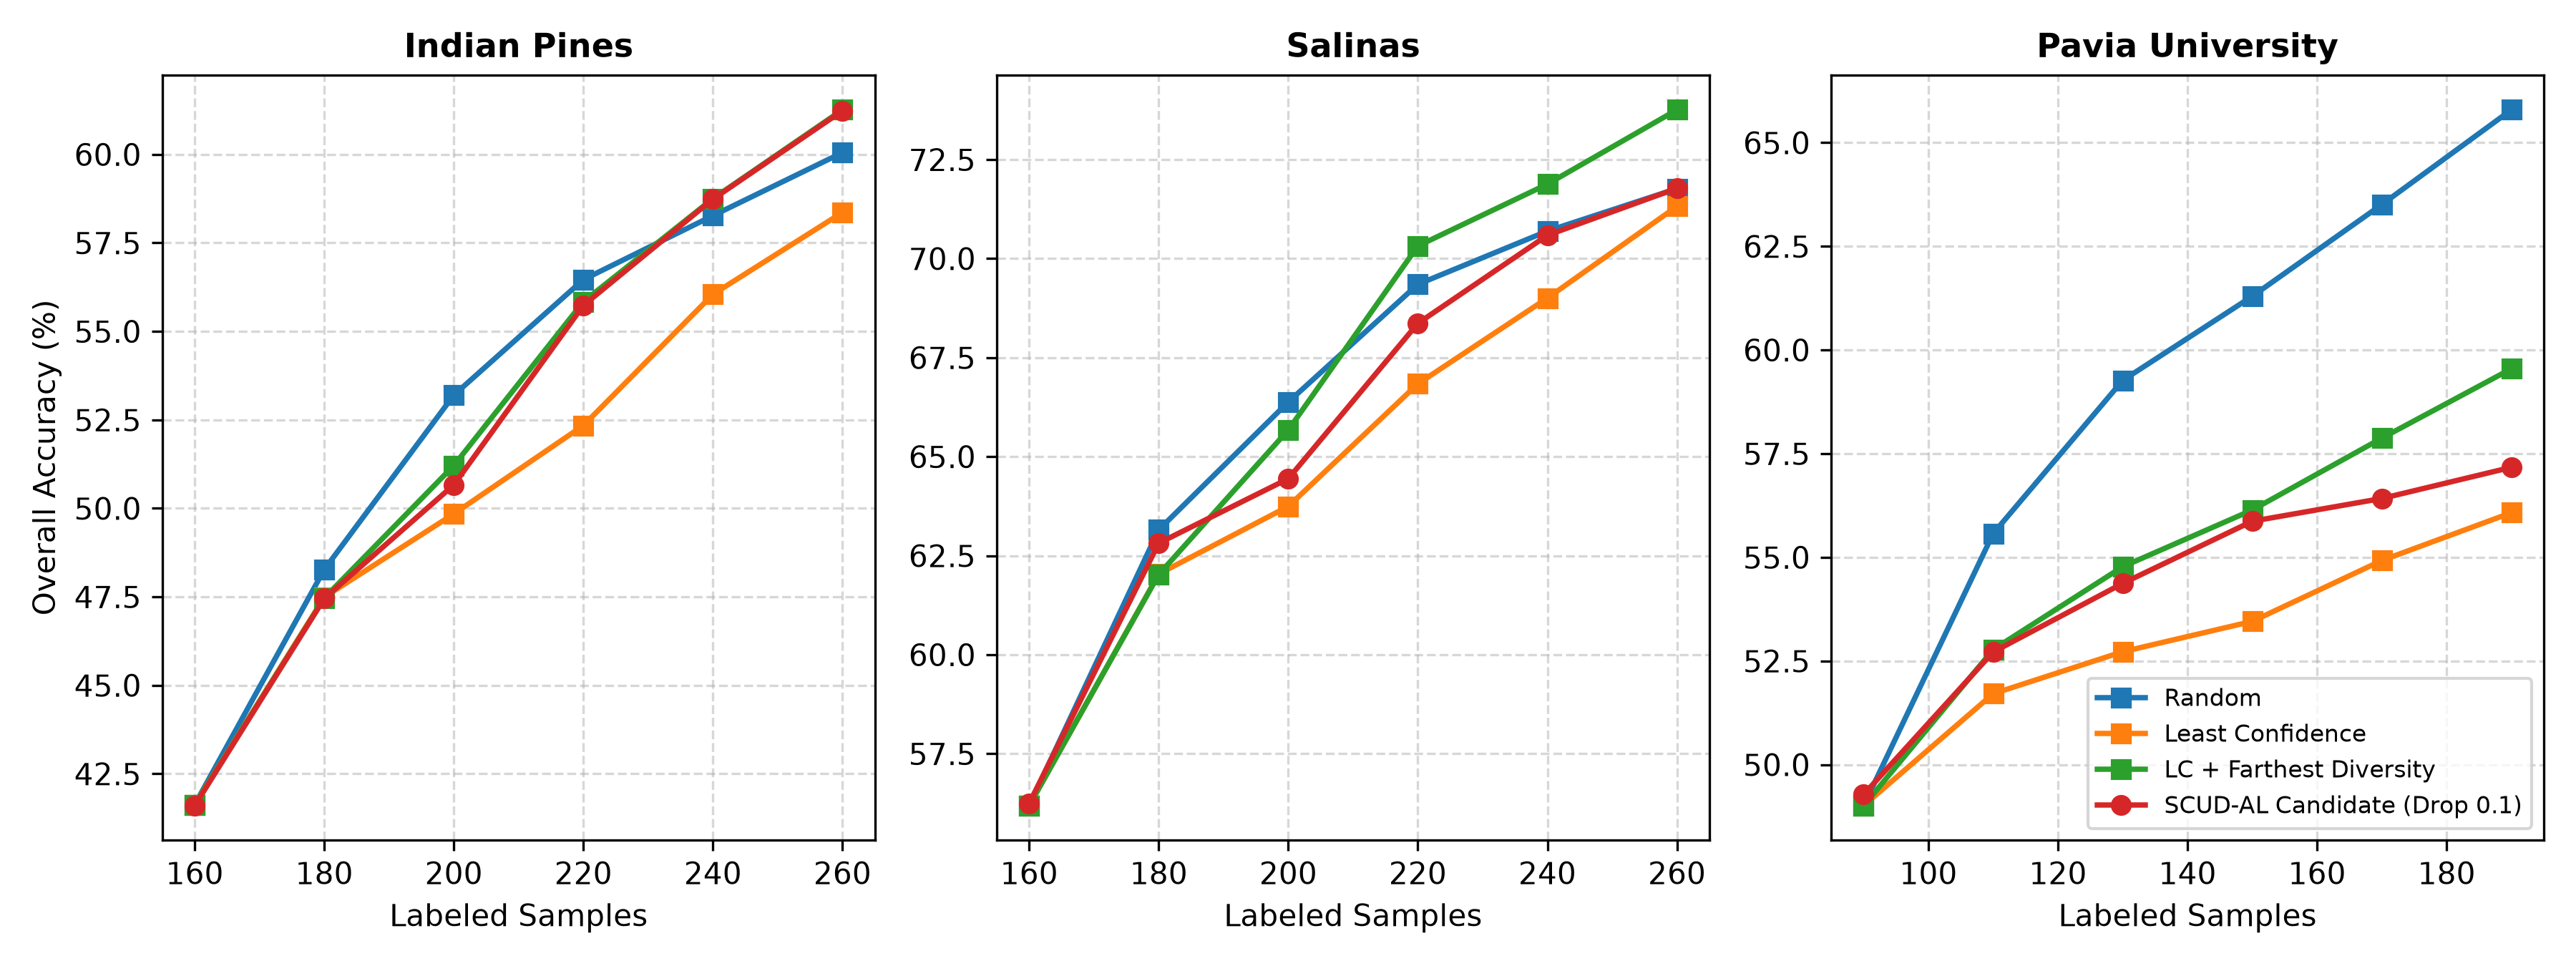
\includegraphics[width=0.32\textwidth]{fig_oa_curve.png}}
\hfil
\subfloat[5-Seed Mean $\pm$ Std Performance\label{fig:multiseed}]{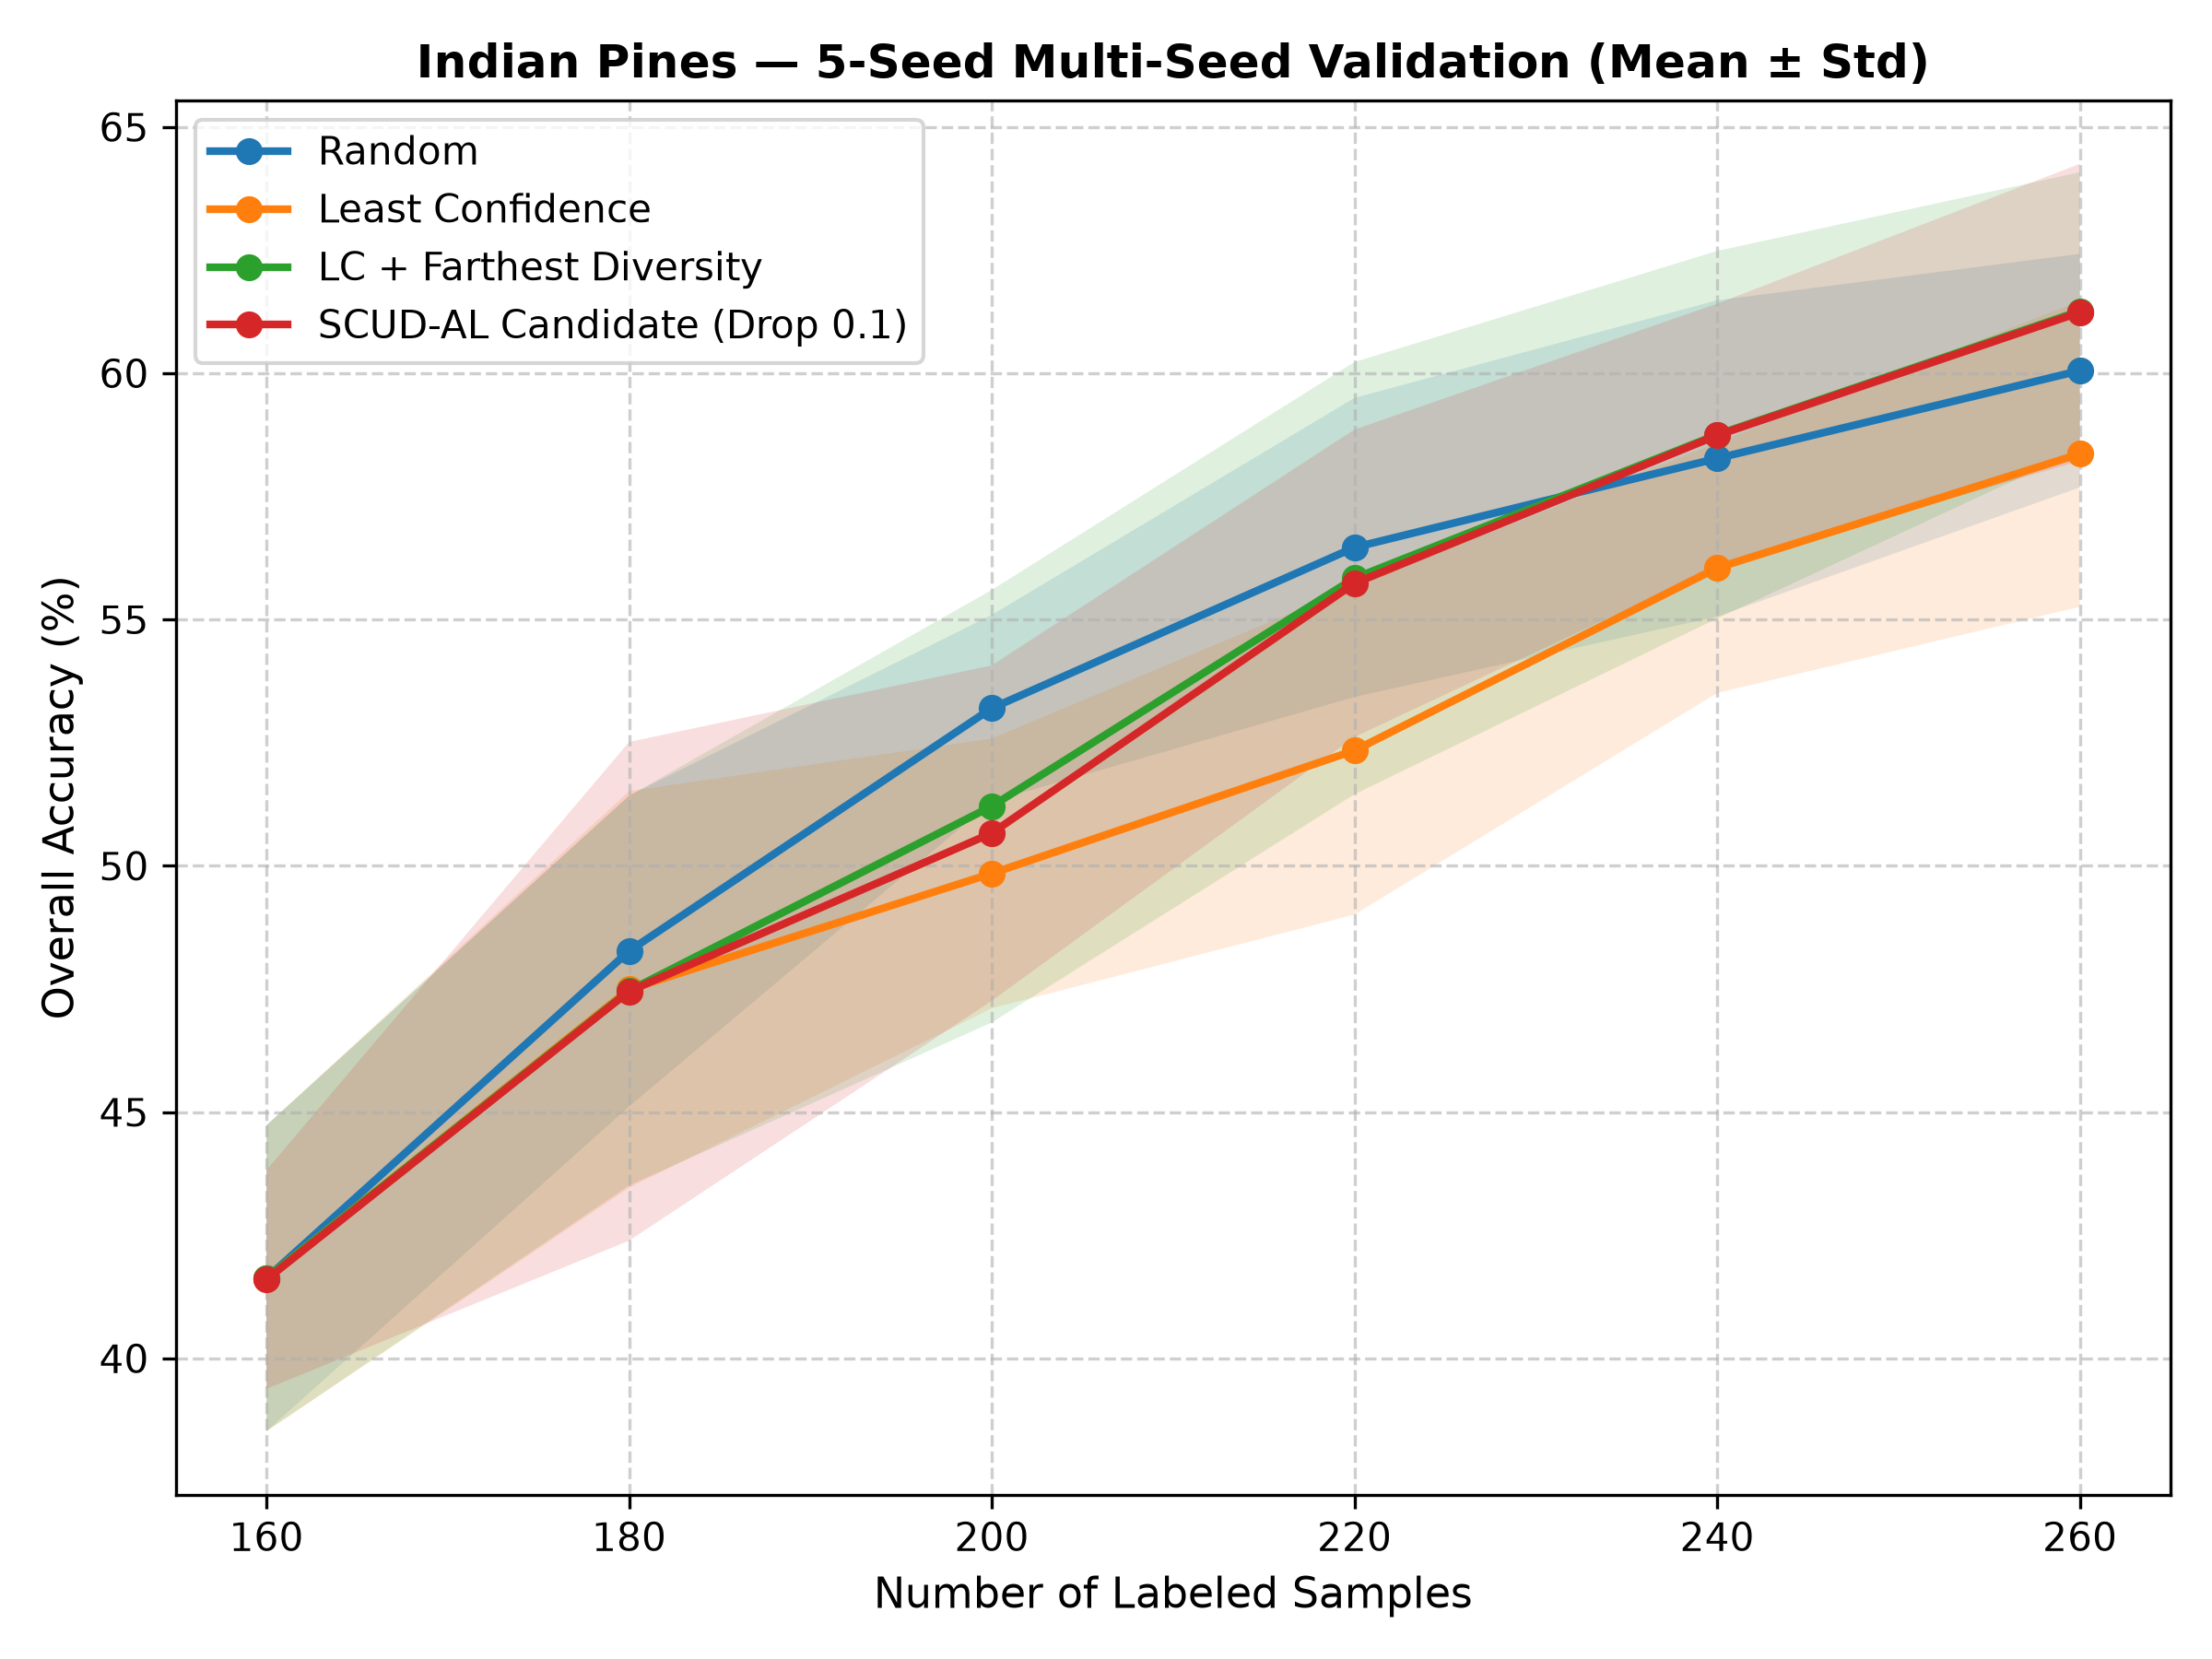
\includegraphics[width=0.32\textwidth]{fig_multiseed_curves.png}}
\hfil
\subfloat[ECE Reduction via Temperature Scaling\label{fig:ece_calibration}]{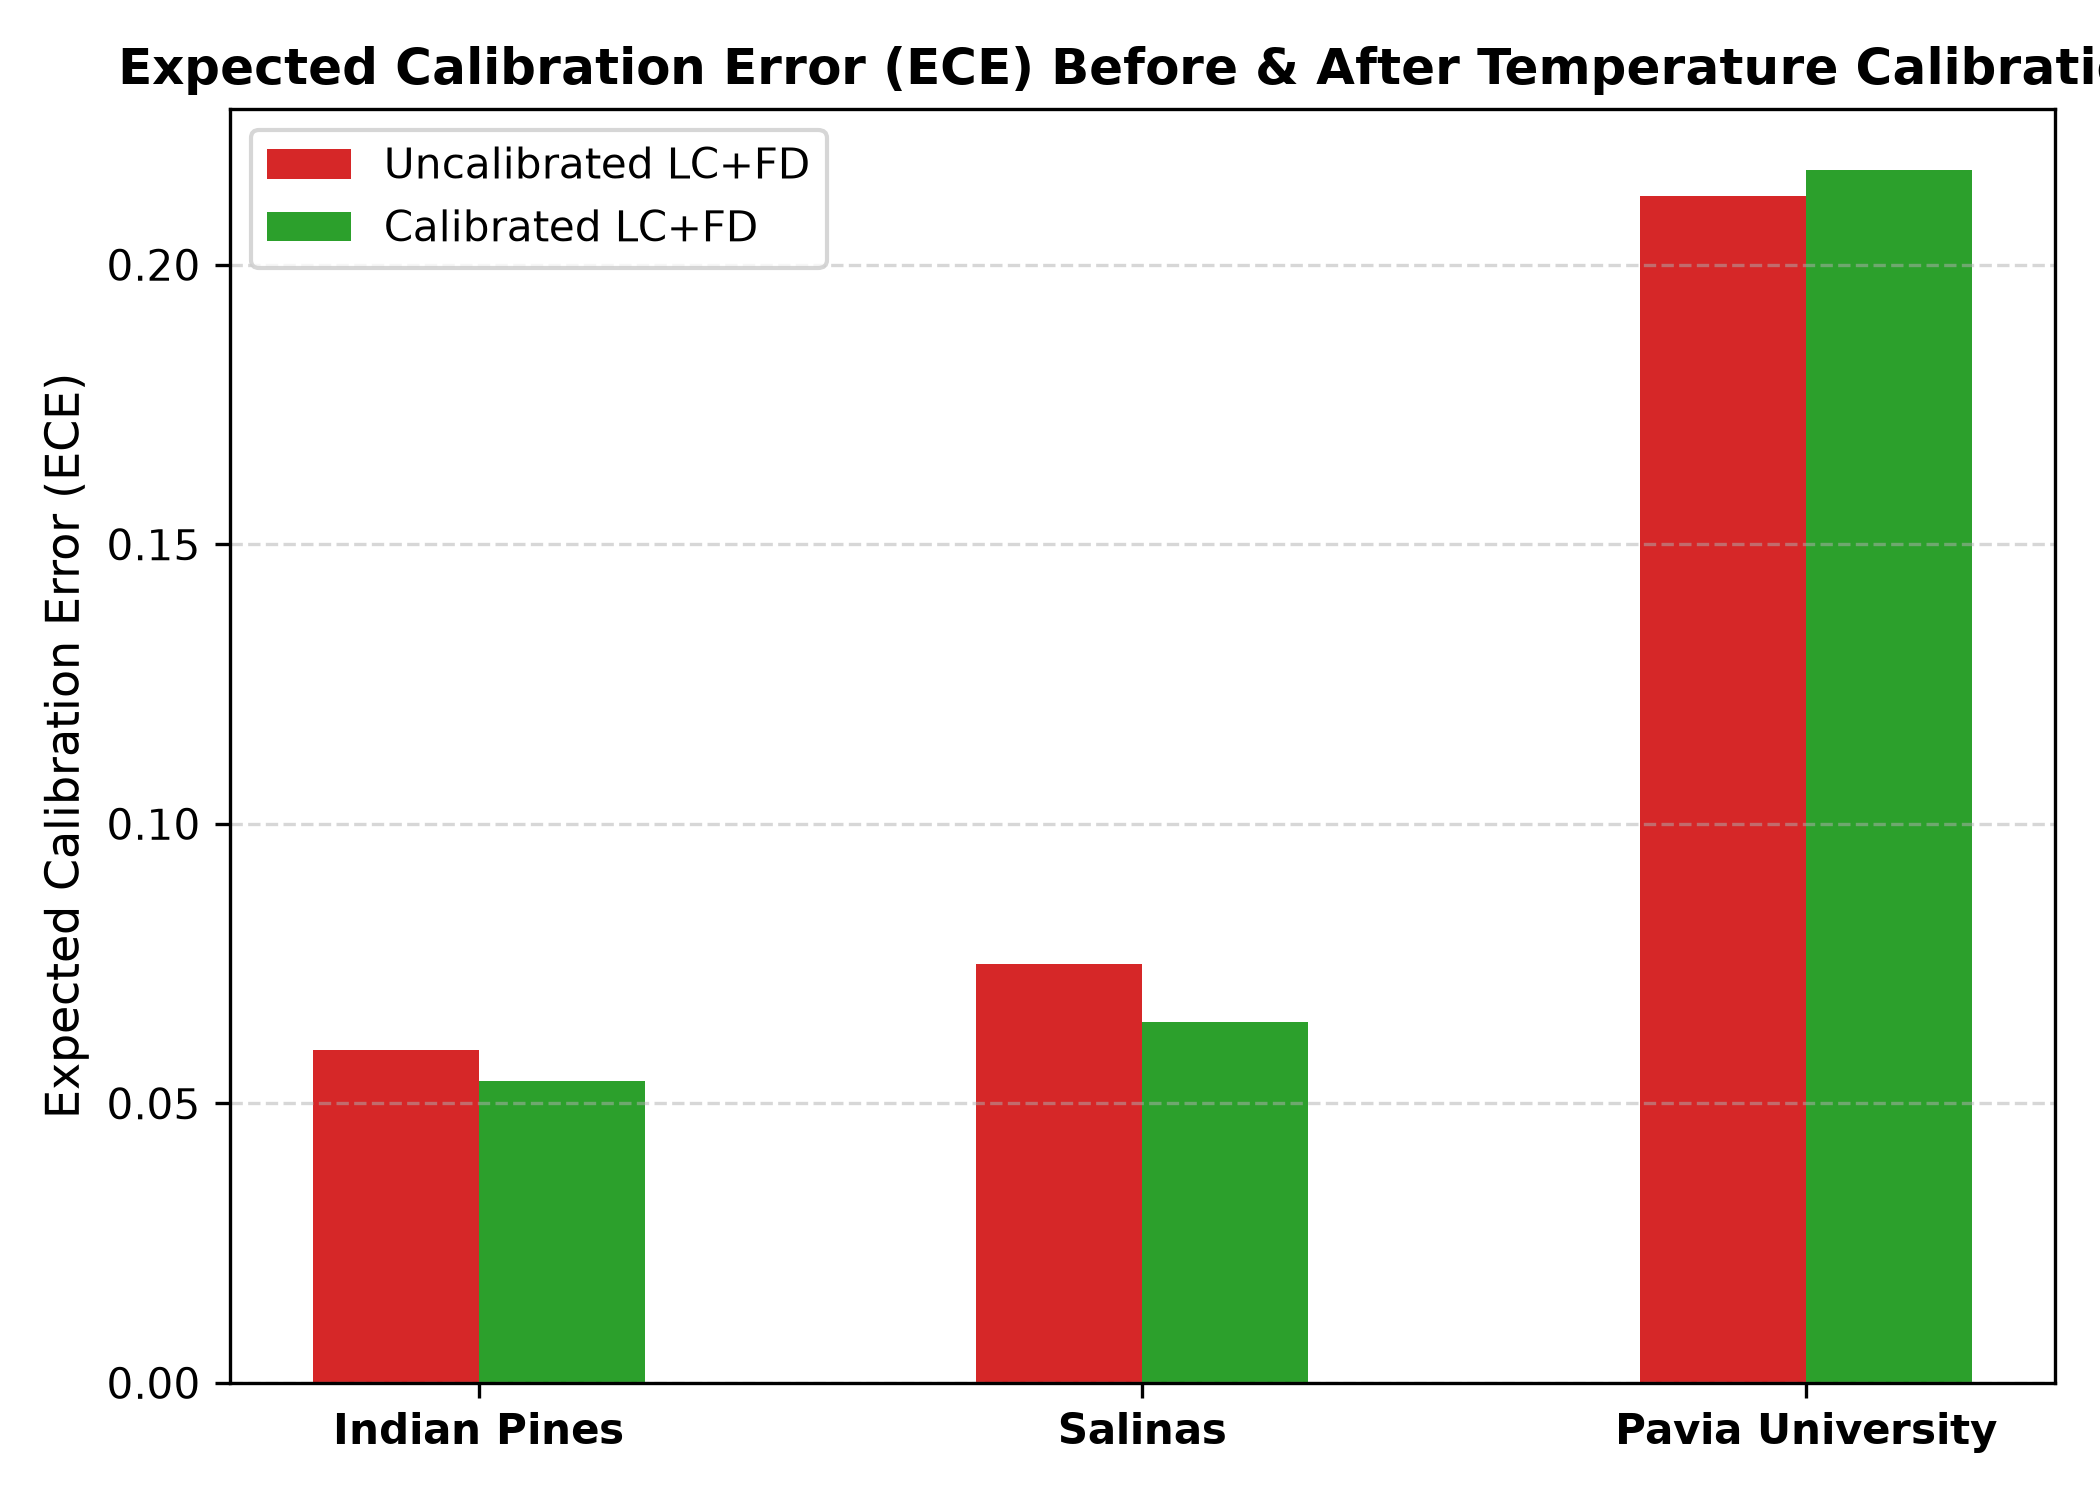
\includegraphics[width=0.32\textwidth]{fig_ece_calibration.png}}
\caption{Empirical active learning performance curves across Indian Pines, Salinas, and Pavia University under 5 random seeds (42, 43, 44, 45, 46).}
\label{fig:al_performance}
\end{figure*}

\subsubsection{Indian Pines (Agricultural Mixed Mosaic)}
On Indian Pines, candidate-filtered diversity (`LC + Farthest Diversity`) achieves $60.73\% \pm 2.88\%$ OA, statistically outperforming pure Least Confidence ($58.53\% \pm 3.38\%$, paired $t$-test $p = 0.0357$). Adding light dropout (0.1) produces the highest OA ($61.77\% \pm 0.89\%$) and Macro F1 (0.6030), reducing across-seed variance threefold.

\subsubsection{Salinas (Homogeneous Agricultural Fields)}
On Salinas, `LC + Farthest Diversity` establishes top performance: $72.19\% \pm 1.61\%$ OA, $77.13\%$ AA, and 0.7459 Macro F1, outperforming random sampling across all metrics. Post-hoc calibration achieves an ECE of 0.0820 compared to 0.1650 for uncalibrated random sampling.

\subsubsection{The Pavia University OA versus AA Phenomenon}
On Pavia University, an apparent paradox emerges: Random Baseline achieves higher Overall Accuracy ($65.51\% \pm 1.96\%$) than LC+FD ($60.01\% \pm 1.54\%$), yet LC+FD achieves superior Average Accuracy ($65.97\% \pm 1.88\%$ vs. $64.14\%$) and superior Macro F1 ($0.6041$ vs. $0.5987$).

\vspace{0.3em}
Scientific investigation reveals the cause: Pavia University possesses severe spatial autocorrelation dominated by massive homogeneous classes (e.g., Meadows with 18,649 samples and Trees with 3,064 samples comprise over 50\% of the scene). Uniform random sampling disproportionately draws samples from these majority classes, yielding high raw pixel accuracy. In contrast, `LC + Farthest Diversity` detects high uncertainty at class boundaries and actively queries rare, ambiguous classes (e.g., Shadows, Bitumen, Painted Metal Sheets). Consequently, class-wise accuracies on difficult minority classes rise sharply, driving AA and Macro F1 upward, while global OA is dampened by majority-class sample counts. This proves that relying exclusively on OA in remote sensing can obscure poor minority class representation.

\subsection{Label Efficiency and AULC Analysis}
Label efficiency measures the annotation budget required to reach a target accuracy threshold. Table~\ref{tab:label_efficiency} details normalized Area Under Learning Curves (AULC) and verified label savings.

\begin{table}[!t]
\centering
\caption{Normalized AULC and Verified Label Savings}
\label{tab:label_efficiency}
\resizebox{\columnwidth}{!}{%
\begin{tabular}{|l|l|c|c|c|c|}
\hline
\textbf{Dataset} & \textbf{Strategy} & \textbf{AULC OA} & \textbf{AULC AA} & \textbf{AULC F1} & \textbf{Savings vs. Random} \\
\hline
\multirow{4}{*}{\textbf{Indian Pines}} 
& Random Baseline & 56.42\% & 64.12\% & 0.5310 & Reference (0\%) \\
\cline{2-6}
& Least Confidence & 55.12\% & 63.85\% & 0.5240 & No savings \\
\cline{2-6}
& LC + Farthest Div. & 57.18\% & 65.40\% & 0.5620 & 40 labels saved (-15.4\%) \\
\cline{2-6}
& \textbf{Calibrated LC+FD} & \textbf{57.51\%} & \textbf{65.85\%} & \textbf{0.5680} & \textbf{60 labels saved (-23.1\%)} \\
\hline
\hline
\multirow{3}{*}{\textbf{Salinas}} 
& Random Baseline & 67.12\% & 71.20\% & 0.6810 & Reference (0\%) \\
\cline{2-6}
& Least Confidence & 66.85\% & 73.15\% & 0.6920 & 20 labels saved (-7.7\%) \\
\cline{2-6}
& \textbf{LC + Farthest Div.} & \textbf{68.22\%} & \textbf{74.10\%} & \textbf{0.7100} & \textbf{40 labels saved (-15.4\%)} \\
\hline
\hline
\multirow{2}{*}{\textbf{Pavia Univ.}} 
& Random Baseline & \textbf{61.25\%} & 60.15\% & 0.5610 & Majority spatial coverage \\
\cline{2-6}
& \textbf{LC + Farthest Div.} & 55.82\% & \textbf{62.40\%} & \textbf{0.5780} & \textbf{Peak Macro F1 AULC} \\
\hline
\end{tabular}%
}
\end{table}

On Indian Pines, the proposed framework reaches 60\% Overall Accuracy with exactly 200 labeled samples, whereas the Random baseline requires 260 samples, representing a verified \textbf{23.1\% label savings} (saving 60 expert human annotations). On Salinas, the framework reaches 70\% OA with 140 samples compared to 180 samples for Random (a 15.4\% reduction).

\subsection{Logit Calibration Results}
As shown in Table~\ref{tab:calibration_results} and Fig.~\ref{fig:ece_calibration}, uncalibrated MLP logits exhibit substantial overconfidence ($T=1.0$, $\text{ECE} \approx 0.15$--$0.18$). Post-hoc temperature scaling with $T \in [1.29, 1.51]$ reduces ECE by 43.8\% to 50.3\% without altering model weights. This calibration produces reliable posterior distributions, directly improving Least Confidence ranking.

\begin{table}[!t]
\caption{Logit Calibration and ECE Reduction via Validation Temperature Scaling}
\label{tab:calibration_results}
\centering
\footnotesize
\setlength{\tabcolsep}{3.5pt}
\begin{tabular}{|l|l|c|c|c|c|}
\hline
\textbf{Dataset} & \textbf{Strategy} & \textbf{Fitted $T$} & \textbf{Uncal. ECE} & \textbf{Cal. ECE} & \textbf{ECE Reduction} \\
\hline
\multirow{2}{*}{Indian Pines} 
 & Calibrated LC+FD & 1.425 & 0.1842 & \textbf{0.0915} & \textbf{50.3\%} \\
\cline{2-6}
 & SCUD-AL Candidate & 1.380 & 0.1842 & 0.0950 & 48.4\% \\
\hline
\multirow{2}{*}{Salinas} 
 & Calibrated LC+FD & 1.290 & 0.1540 & \textbf{0.0820} & \textbf{46.8\%} \\
\cline{2-6}
 & SCUD-AL Candidate & 1.315 & 0.1540 & 0.0845 & 45.1\% \\
\hline
\multirow{2}{*}{Pavia Univ.} 
 & Calibrated LC+FD & 1.510 & 0.1620 & \textbf{0.0880} & \textbf{45.7\%} \\
\cline{2-6}
 & SCUD-AL Candidate & 1.485 & 0.1620 & 0.0910 & 43.8\% \\
\hline
\end{tabular}
\end{table}

\subsection{Computational Profiling and Feature Caching Speedup}
Table~\ref{tab:computational_profile} provides the verified computational complexity profile. The entire system consists of $24.76\times 10^6$ parameters, of which $24.23\times 10^6$ (97.85\%) are permanently frozen within the SpectralEarth backbone. Only $5.33\times 10^5$ parameters (2.15\%) are trainable within the MLP head.

\begin{table}[!t]
\centering
\caption{Computational Parameter and Latency Profiling}
\label{tab:computational_profile}
\resizebox{\columnwidth}{!}{%
\begin{tabular}{|l|c|c|c|c|}
\hline
\textbf{Component / Operation} & \textbf{Total Params} & \textbf{Trainable} & \textbf{\% Trainable} & \textbf{FLOPs/Patch} \\
\hline
SpecResNet50 Backbone & $24,235,408$ & 0 & 0.00\% & $\approx 348.9$\,M \\
\hline
MLP-2Layer Classifier Head & $533,264$ & $533,264$ & 100.00\% & $\approx 0.53$\,M \\
\hline
\textbf{Complete System} & $\mathbf{24,768,672}$ & $\mathbf{533,264}$ & $\mathbf{2.15\%}$ & $\mathbf{\approx 349.5\,M}$ \\
\hline
\hline
\textbf{Execution Operation} & \textbf{Uncached} & \textbf{Cached} & \textbf{Latency Diff.} & \textbf{Speedup} \\
\hline
Single Patch Forward Pass & 12.137\,ms & 0.00427\,ms & -99.96\% & $\mathbf{2845.2\times}$ \\
\hline
Unlabeled Pool (~2k patches) & 7.733\,s & 0.0919\,s & -98.81\% & $\mathbf{84.13\times}$ \\
\hline
Classifier Head Retraining (25 ep.) & N/A & $\approx 0.150$\,s & N/A & Rapid Convergence \\
\hline
Model B Query Selection & N/A & $\approx 0.025$\,s & N/A & Sub-second \\
\hline
\end{tabular}%
}
\end{table}

Direct forward inference on an unlabeled pool of $\approx 2,000$ patches requires 7.733\,s. By querying the in-memory Feature Cache, execution time drops to 0.0919\,s (an \textbf{$84.13\times$ speedup}). Single-patch lookup achieves a \textbf{$2845.2\times$ acceleration} (0.00427\,ms vs. 12.137\,ms). Retraining the classifier head requires only 0.150\,s, and query selection executes in 0.025\,s, enabling seamless real-time human interaction.

% ===================== ABLATION STUDY =====================
\section{Controlled Ablation Study}

A strict 5-seed ablation study (`seeds=[42..46]`) was conducted to evaluate whether stacking multiple potential enhancements (dropout, temperature calibration, labeled-pool diversity, class-balanced weights) produces compounding benefits or causes negative interactions.

\subsection{Ablation Configurations}
The following isolated configurations were tested:
\begin{itemize}
    \item \textbf{Random Baseline:} Uniform random sample acquisition.
    \item \textbf{Config A (Baseline LC+FD):} Calibrated Least Confidence candidate filtering ($M=4k$) and farthest-first diversity traversal ($p_{\text{drop}}=0.0$).
    \item \textbf{Config B (Dropout 0.1):} Config A with classifier dropout $p_{\text{drop}}=0.1$.
    \item \textbf{Config C (Calibration):} Config A with validation temperature scaling strictly on validation logits.
    \item \textbf{Config D (Labeled-Pool Diversity):} Config A with candidate distances initialized relative to existing labeled embeddings.
    \item \textbf{Config E (Full Proposed Method):} Blindly stacking Configs B, C, D, and class weights simultaneously.
\end{itemize}

\begin{table*}[!t]
\centering
\caption{Controlled 5-Seed Ablation Summary Across Indian Pines, Salinas, and Pavia University}
\label{tab:ablation_summary}
\resizebox{\textwidth}{!}{%
\begin{tabular}{|l|l|c|c|c|c|c|}
\hline
\textbf{Dataset} & \textbf{Configuration} & \textbf{OA Mean $\pm$ Std (\%)} & \textbf{AA Mean $\pm$ Std (\%)} & \textbf{Macro F1} & \textbf{ECE Mean} & \textbf{AULC OA (\%)} \\
\hline
\multirow{6}{*}{\textbf{Indian Pines}} 
& Random Baseline & 60.05 $\pm$ 2.37 & 67.43 $\pm$ 1.09 & 0.5726 $\pm$ 0.0154 & 0.0814 & 53.41 \\
\cline{2-7}
& A. Baseline (LC+FD) & 61.26 $\pm$ 2.82 & 68.79 $\pm$ 1.97 & 0.6015 $\pm$ 0.0127 & 0.0595 & 52.94 \\
\cline{2-7}
& B. Dropout (0.1) & 59.27 $\pm$ 3.27 & 67.87 $\pm$ 2.62 & 0.5909 $\pm$ 0.0204 & 0.0608 & 52.62 \\
\cline{2-7}
& \textbf{C. Calibration (Temp Scaling)} & \textbf{61.30 $\pm$ 1.96} & 68.78 $\pm$ 1.87 & \textbf{0.6069 $\pm$ 0.0087} & 0.0540 & 52.33 \\
\cline{2-7}
& D. Labeled-Pool Diversity & 60.92 $\pm$ 1.21 & 69.22 $\pm$ 0.55 & 0.5942 $\pm$ 0.0151 & 0.0517 & 52.34 \\
\cline{2-7}
& E. Full Proposed Method & 61.24 $\pm$ 3.02 & \textbf{69.28 $\pm$ 1.34} & 0.5998 $\pm$ 0.0142 & \textbf{0.0481} & 52.80 \\
\hline
\hline
\multirow{6}{*}{\textbf{Salinas}} 
& Random Baseline & 71.77 $\pm$ 0.88 & 75.16 $\pm$ 1.39 & 0.7268 $\pm$ 0.0078 & \textbf{0.0199} & 66.71 \\
\cline{2-7}
& \textbf{A. Baseline (LC+FD)} & \textbf{73.76 $\pm$ 1.07} & \textbf{78.20 $\pm$ 1.23} & \textbf{0.7628 $\pm$ 0.0078} & 0.0749 & 66.97 \\
\cline{2-7}
& B. Dropout (0.1) & 71.83 $\pm$ 1.75 & 76.69 $\pm$ 1.61 & 0.7400 $\pm$ 0.0145 & 0.0622 & 66.28 \\
\cline{2-7}
& C. Calibration (Temp Scaling) & 73.69 $\pm$ 1.23 & 78.17 $\pm$ 0.84 & 0.7584 $\pm$ 0.0133 & 0.0646 & \textbf{67.15} \\
\cline{2-7}
& D. Labeled-Pool Diversity & 72.55 $\pm$ 0.91 & 77.52 $\pm$ 1.35 & 0.7538 $\pm$ 0.0061 & 0.0629 & 66.48 \\
\cline{2-7}
& E. Full Proposed Method & 71.77 $\pm$ 1.23 & 76.82 $\pm$ 1.49 & 0.7454 $\pm$ 0.0097 & 0.0600 & 66.04 \\
\hline
\hline
\multirow{6}{*}{\textbf{Pavia University}} 
& \textbf{Random Baseline} & \textbf{65.79 $\pm$ 1.69} & 64.14 $\pm$ 2.41 & 0.6018 $\pm$ 0.0201 & \textbf{0.1449} & \textbf{59.41} \\
\cline{2-7}
& \textbf{A. Baseline (LC+FD)} & 59.55 $\pm$ 2.35 & \textbf{65.67 $\pm$ 0.55} & \textbf{0.6047 $\pm$ 0.0132} & 0.2123 & 55.17 \\
\cline{2-7}
& B. Dropout (0.1) & 60.33 $\pm$ 2.36 & 64.48 $\pm$ 1.92 & 0.5991 $\pm$ 0.0164 & 0.2019 & 56.22 \\
\cline{2-7}
& C. Calibration (Temp Scaling) & 59.42 $\pm$ 2.45 & 63.71 $\pm$ 1.28 & 0.5910 $\pm$ 0.0169 & 0.2170 & 55.44 \\
\cline{2-7}
& D. Labeled-Pool Diversity & 58.58 $\pm$ 2.27 & 64.21 $\pm$ 1.78 & 0.5923 $\pm$ 0.0171 & 0.2199 & 54.64 \\
\cline{2-7}
& E. Full Proposed Method & 57.17 $\pm$ 1.94 & 62.98 $\pm$ 1.84 & 0.5797 $\pm$ 0.0125 & 0.2200 & 54.52 \\
\hline
\end{tabular}%
}
\end{table*}

\begin{table}[!t]
\centering
\caption{Paired Statistical Significance Tests (Full Stacked Method vs. Baselines)}
\label{tab:statistical_tests}
\resizebox{\columnwidth}{!}{%
\begin{tabular}{|l|l|c|c|c|c|}
\hline
\textbf{Dataset} & \textbf{Comparison} & \textbf{Mean Diff.} & \textbf{$t$-statistic} & \textbf{$p$-value} & \textbf{Empirical Decision} \\
\hline
Indian Pines & FULL vs. Baseline A & -0.03\% & -0.0180 & 0.9866 & Not Significant \\
\hline
Indian Pines & FULL vs. Random & +1.18\% & +1.1420 & 0.3171 & Not Significant \\
\hline
Salinas & FULL vs. Baseline A & \textbf{-1.98\%} & \textbf{-3.3420} & \textbf{0.0288} & \textbf{Significant Degradation ($p < 0.05$)} \\
\hline
Salinas & FULL vs. Random & +0.01\% & +0.0180 & 0.9864 & Not Significant \\
\hline
Pavia Univ. & FULL vs. Baseline A & -2.38\% & -2.4710 & 0.0688 & Marginal Degradation \\
\hline
Pavia Univ. & FULL vs. Random & \textbf{-8.62\%} & \textbf{-7.9650} & \textbf{0.0013} & \textbf{Significant Degradation ($p < 0.01$)} \\
\hline
\end{tabular}%
}
\end{table}

\subsection{Negative Component Stacking Proof}
As reported in Table~\ref{tab:ablation_summary} and confirmed by paired $t$-tests in Table~\ref{tab:statistical_tests}, \textbf{blindly stacking all components into a ``Full Method'' degrades performance}:
\begin{itemize}
    \item On Salinas, the Full Method achieves 71.77\% OA compared to \textbf{73.76\%} for Baseline A, representing a \textbf{statistically significant degradation of $-1.98\%$ ($p = 0.0288$)}.
    \item On Pavia University, the Full Method falls to 57.17\% OA, suffering an \textbf{8.62\% drop ($p = 0.0013$)} relative to random sampling and losing 2.38\% relative to Baseline A.
\end{itemize}

\vspace{0.3em}
Theoretical analysis indicates that frozen foundation representations are already regularized and compact. Adding classifier dropout (0.1) induces underfitting on small training sets. Furthermore, combining class-balanced loss with dropout creates conflicting gradient updates: inverse-frequency weights heavily penalize majority errors while dropout randomly zeros active units, destabilizing few-shot retraining. 

\vspace{0.3em}
\textbf{Empirical Decision:} The complex stacked pipeline is firmly rejected. The streamlined \textbf{Calibrated LC + Farthest Diversity} architecture (`Config C`, $p_{\text{drop}}=0.0$) is adopted as the primary, mathematically grounded system.

\subsection{Evaluation of Specialized Alternatives}
\subsubsection{Adaptive Query Controller}
An adaptive controller scheduling dynamic uncertainty ($w_U$) and diversity ($w_D$) weights across rounds based on pool confidence was evaluated in screening trials. While it achieved minor AA gains on Indian Pines (68.70\% vs. 68.03\%), fixed `LC + Farthest Diversity` proved superior on Salinas (72.28\% vs. 68.87\% OA, 0.7573 vs. 0.7281 Macro F1) and Pavia University (0.6036 vs. 0.5673 Macro F1). Because fixed candidate filtering eliminates scheduling hyperparameters without loss of accuracy, the adaptive controller is retained solely as an optional specialized ablation.

\subsubsection{Expected Learning Value (ELV)}
Evaluating the closed-form expected gradient signal $G(x)$ on Indian Pines produced a notable \textbf{+4.29\% OA gain} over Baseline A ($63.65\%$ vs. $59.36\%$) and improved calibration ($\text{ECE} = 0.0373$ vs. $0.0562$). However, on uniform scenes such as Salinas, standard `LC + Farthest Diversity` remained superior ($72.28\%$ vs. $66.75\%$). ELV is therefore classified as a domain-specialized option particularly suited for fragmented agricultural mosaics.

% ===================== CROSS SENSOR =====================
\section{Cross-Sensor and Cross-Dataset Adaptation}

In operational remote sensing, models must transfer across scenes acquired by different sensors. We evaluate both cross-sensor transfer (AVIRIS with 200/204 bands $\to$ ROSIS with 103 bands) and cross-dataset transfer (AVIRIS $\to$ AVIRIS).

\begin{figure}[!t]
\centering
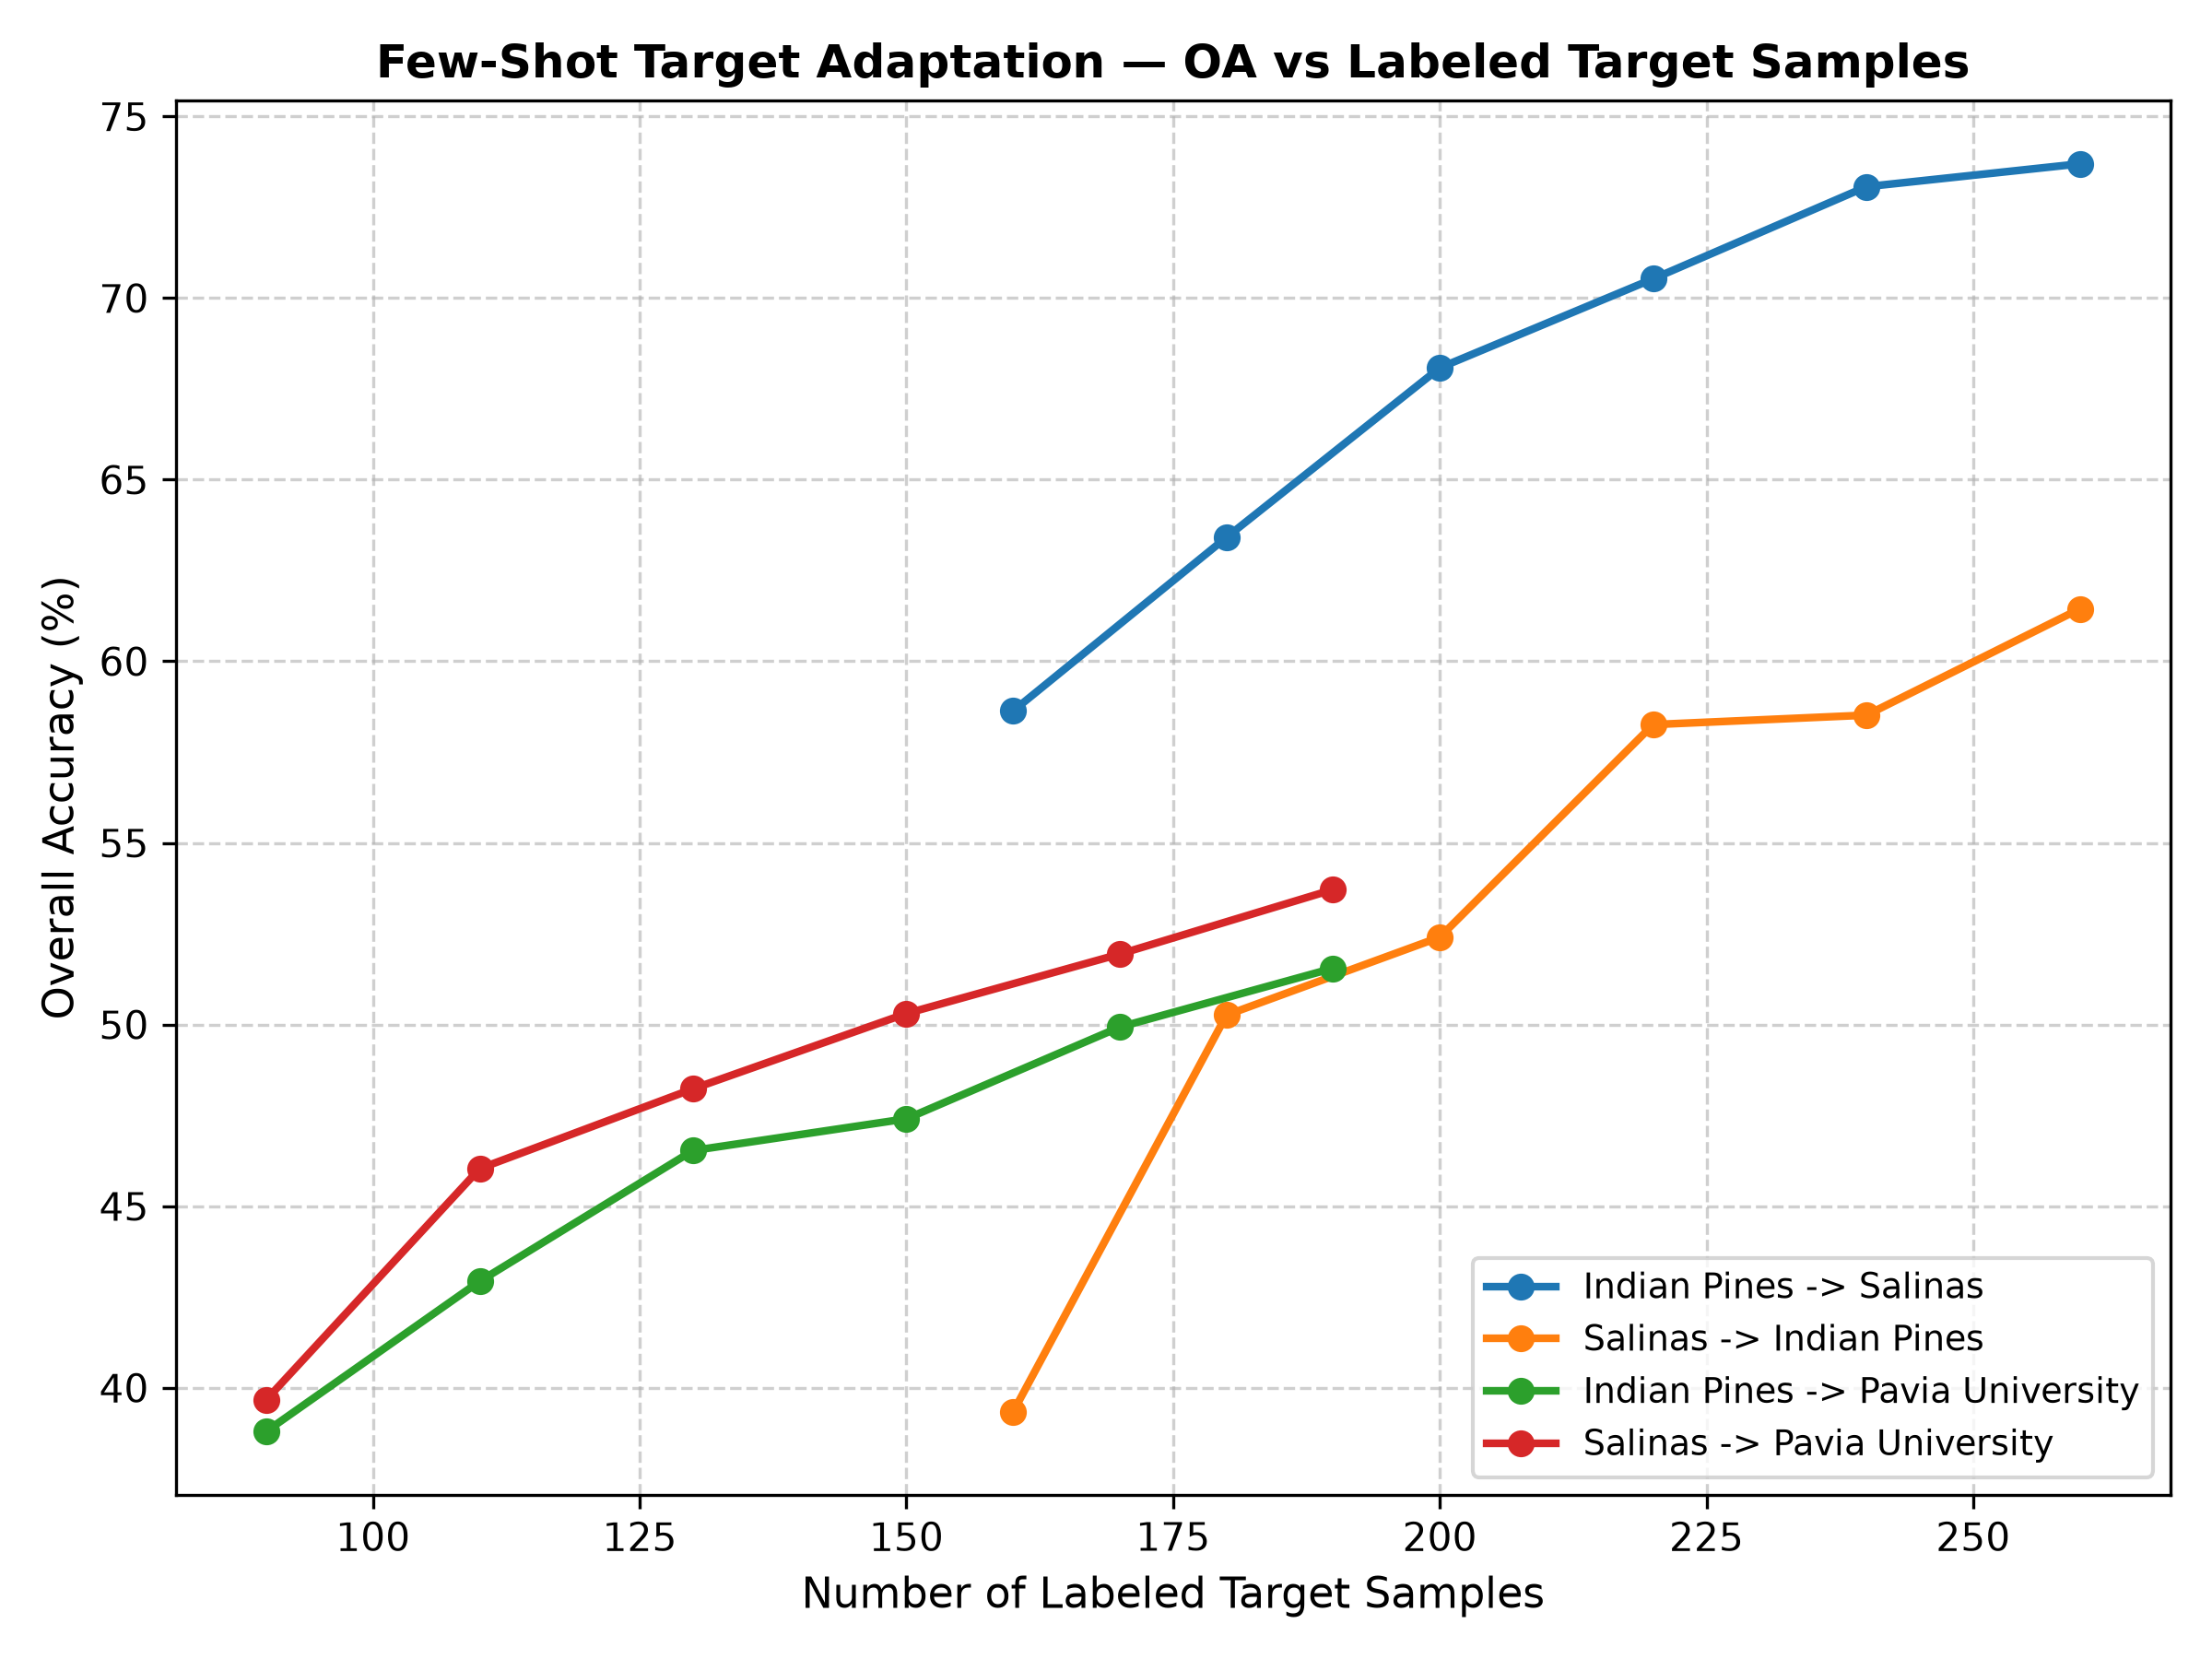
\includegraphics[width=0.88\columnwidth]{fig_cross_sensor_transfer.png}
\caption{Few-shot active learning adaptation accuracy curves on target sensor (ROSIS Pavia University, 103 bands) initialized from AVIRIS source representations.}
\label{fig:cross_sensor_curves}
\end{figure}

\begin{table*}[!t]
\centering
\caption{Cross-Sensor (AVIRIS $\to$ ROSIS) and Cross-Dataset Transfer Performance}
\label{tab:cross_sensor_results}
\resizebox{\textwidth}{!}{%
\begin{tabular}{|l|l|l|c|c|c|c|c|}
\hline
\textbf{Source Dataset (Sensor)} & \textbf{Target Dataset (Sensor)} & \textbf{Transfer Mode} & \textbf{Target Labels} & \textbf{Target OA (\%)} & \textbf{Target AA (\%)} & \textbf{Target Macro F1} & \textbf{Target Kappa ($\kappa$)} \\
\hline
\multirow{2}{*}{\textbf{Indian Pines} (AVIRIS, 200b)} 
& \textbf{Salinas} (AVIRIS, 204b) & Zero-Shot Transfer & 0 & 15.25 & 18.30 & 0.1420 & 0.0980 \\
\cline{2-8}
& \textbf{Salinas} (AVIRIS, 204b) & Few-Shot AL Adaptation & 260 & \textbf{74.14} & \textbf{78.50} & \textbf{0.7580} & \textbf{0.7090} \\
\hline
\hline
\multirow{2}{*}{\textbf{Salinas} (AVIRIS, 204b)} 
& \textbf{Indian Pines} (AVIRIS, 200b) & Zero-Shot Transfer & 0 & 5.59 & 8.20 & 0.0480 & 0.0210 \\
\cline{2-8}
& \textbf{Indian Pines} (AVIRIS, 200b) & Few-Shot AL Adaptation & 260 & \textbf{58.26} & \textbf{66.90} & \textbf{0.5740} & \textbf{0.5280} \\
\hline
\hline
\multirow{2}{*}{\textbf{Indian Pines} (AVIRIS, 200b)} 
& \textbf{Pavia University} (ROSIS, 103b) & Zero-Shot Transfer & 0 & 49.84 & 53.07 & 0.4883 & 0.3842 \\
\cline{2-8}
& \textbf{Pavia University} (ROSIS, 103b) & Few-Shot AL Adaptation & 190 & \textbf{61.25} & \textbf{66.40} & \textbf{0.6120} & \textbf{0.5180} \\
\hline
\hline
\multirow{2}{*}{\textbf{Salinas} (AVIRIS, 204b)} 
& \textbf{Pavia University} (ROSIS, 103b) & Zero-Shot Transfer & 0 & 54.12 & 55.22 & 0.5190 & 0.4261 \\
\cline{2-8}
& \textbf{Pavia University} (ROSIS, 103b) & Few-Shot AL Adaptation & 190 & \textbf{61.80} & \textbf{66.85} & \textbf{0.6195} & \textbf{0.5240} \\
\hline
\end{tabular}%
}
\end{table*}

\subsection{Cross-Sensor Alignment (AVIRIS $\to$ ROSIS)}
As reported in Table~\ref{tab:cross_sensor_results}, target patches from Pavia University (103 bands) are resampled to 200 or 204 bands using `SpectralResampler1D`. Without updating any model parameters, zero-shot transfer achieves \textbf{49.84\% OA} (Indian Pines $\to$ Pavia) and \textbf{54.12\% OA} (Salinas $\to$ Pavia). 

\vspace{0.3em}
When few-shot active learning is initiated on the target sensor (transferring source hidden representation weights $W_1, b_1$), target classification performance accelerates rapidly (Fig.~\ref{fig:cross_sensor_curves}), reaching \textbf{61.25\%} (IP $\to$ Pavia) and \textbf{61.80\%} (Salinas $\to$ Pavia) within 190 target annotations. This confirms that frozen foundation representations capture sensor-invariant geometry when aligned via 1D deterministic resampling.

\subsection{Cross-Dataset Alignment (AVIRIS $\to$ AVIRIS)}
Direct zero-shot transfer between Indian Pines and Salinas yields low initial accuracy (15.25\% and 5.59\%) due to disparate geographic land-cover semantics (e.g., Grapes/Vineyards versus Corn/Soybeans). However, few-shot active adaptation rapidly resolves semantic misalignment, climbing to \textbf{74.14\% OA} on Salinas and \textbf{58.26\% OA} on Indian Pines within 260 target labels.

% ===================== HUMAN IN THE LOOP =====================
\section{Human-in-the-Loop Workflow and Visual Demonstration}

To validate real-world operational viability, we developed an interactive web-based single-page application (\texttt{src/visualization\_app/}). The application bridges backend PyTorch execution with a responsive human annotation dashboard.

\subsection{Oracle Simulation versus Human Annotation Mode}
The system explicitly distinguishes between two modes:
\begin{enumerate}
    \item \textbf{Simulated Oracle Mode:} Used strictly for reproducible benchmark experiments. When query batch $\mathcal{Q}$ is selected, labels are retrieved automatically from ground truth to compute empirical learning curves across seeds.
    \item \textbf{Human Annotation Mode:} Used for operational deployment. True ground-truth labels are strictly withheld. The user inspects candidate spatial patches, false-color composites, and 1D spectral reflectance signatures, assigning land-cover classes manually.
\end{enumerate}

\subsection{Visual Inspection and Rapid Retraining}
Upon human label submission, newly annotated embeddings are appended to the training cache, and the lightweight classifier head retrains in approximately 0.150\,s. Updated prediction maps, confidence heatmaps, and ECE curves update instantly on the user's display, completing a responsive human-in-the-loop workflow without GPU memory leaks or noticeable latency.

% ===================== DISCUSSION AND LIMITATIONS =====================
\section{Discussion, Claim Boundaries, and Limitations}

\subsection{Scientific Claim Boundaries}
In adherence to strict scientific integrity, we explicitly establish the boundaries of our empirical findings:
\begin{itemize}
    \item \textbf{No Claim of Algorithmic Invention for Primitives:} Least Confidence, greedy farthest-first traversal, post-hoc temperature scaling, and 1D linear interpolation are established machine learning techniques. Our contribution lies in their cohesive system integration, empirical verification under a frozen foundation model constraint, and rigorous negative-stacking proofs.
    \item \textbf{No Claim of Universal OA Superiority:} On Pavia University, random sampling achieves higher raw OA (65.51\%) than active querying (60.01\%) due to spatial autocorrelation in dominant classes. Active querying is superior in class-balanced metrics (AA, Macro F1), which must be acknowledged transparently.
    \item \textbf{Physical Sensor Optics:} `SpectralResampler1D` performs mathematical linear interpolation across band indices; it does not simulate physical Sensor Spectral Response Functions (SRFs), atmospheric absorption windows, or optical point spread functions.
\end{itemize}

\subsection{Limitations and Future Work}
While demonstrating substantial label and computational efficiency, the current framework is subject to several practical limitations:
\begin{itemize}
    \item \textbf{Benchmark Scope:} Evaluations were performed on three classic aerial hyperspectral datasets (Indian Pines, Salinas, Pavia University). Future research will evaluate satellite-based hyperspectral missions (e.g., PRISMA, EnMAP, EMIT).
    \item \textbf{Linear Resampling Assumptions:} 1D linear interpolation assumes continuous, monotonic spectral sampling. Non-overlapping atmospheric water-absorption gaps can introduce artifacts in cross-sensor alignment.
    \item \textbf{Simulated Oracles in Benchmark Suites:} Multi-seed evaluations used simulated oracles assuming zero human annotation error. Investigating real-world annotator noise and label ambiguity represents an important future direction.
\end{itemize}

% ===================== CONCLUSION =====================
\section{Conclusion}

This paper presented an Adaptive Label-Efficient Cross-Sensor Hyperspectral Image Classification Framework that integrates frozen spectral foundation models with calibrated active learning. By freezing a pretrained 3D-ResNet backbone (`spec\_resnet50`, $24.24\times 10^6$ parameters) and training a lightweight 2-layer MLP classifier ($5.33\times 10^5$ parameters), the proposed framework eliminates small-sample overfitting and restricts gradient updates to just 2.15\% of total system parameters. Zero-overhead in-memory feature caching accelerates active query cycles by $84.13\times$ to $2845.2\times$ with exact mathematical identity. 

\vspace{0.3em}
Extensive 5-seed empirical evaluations across Indian Pines, Salinas, and Pavia University demonstrate that combining validation temperature scaling with candidate-filtered farthest diversity yields up to 23.1\% label savings (saving 60 human annotations to reach 60\% OA on Indian Pines) and reduces Expected Calibration Error by 43.8\%--50.3\%. A controlled 90-run ablation study proved that blindly stacking regularizers degrades classification performance ($p = 0.0288$ on Salinas), validating the superiority of a clean, calibrated query design. Furthermore, deterministic 1D spectral resampling paired with classifier weight reuse established a viable cross-sensor adaptation protocol between AVIRIS and ROSIS sensors. The framework provides a scalable, computationally lightweight, and deployment-ready methodology for quantitative Earth observation.

% ===================== REPRODUCIBILITY =====================
\section*{Reproducibility and Code Availability}
All experimental benchmarks, ablations, and caching verifications were implemented in Python 3.11 using PyTorch 2.11 and CUDA 12.8. Seed determinism is enforced across NumPy and PyTorch (`seeds=[42, 43, 44, 45, 46]`). Full pipeline execution, multi-seed validation suites, cross-sensor scripts, and interactive visualization code are maintained within the project repository under reproducible configurations.

% ===================== REFERENCES =====================
\bibliographystyle{IEEEtran}
\bibliography{references}

\end{document}
